% =====================================================================
%  Exact Minimum Measurement Dependence for Violating the CHSH Inequality
%  Target: Phys. Rev. A (revtex4-2). Compile: pdflatex main; bibtex main;
%  pdflatex main; pdflatex main   (supplement is a separate document, supp.tex)
% =====================================================================
\documentclass[aps,pra,reprint,superscriptaddress,floatfix]{revtex4-2}

\usepackage{amsmath,amssymb}
\usepackage{amsthm}
\usepackage{booktabs}
\usepackage{array}
\usepackage{graphicx}

\newcommand{\TV}{\mathrm{TV}}
\newtheorem{lemma}{Lemma}
\newtheorem{theorem}{Theorem}
\newtheorem{proposition}{Proposition}

\begin{document}

% TODO: replace with real author block (name, affiliation, email) before submission.
\title{Exact minimum measurement dependence for violating the CHSH inequality}
\author{Dan Petersen}
\noaffiliation

\date{\today}

\begin{abstract}
How much measurement dependence must a local hidden-variable model have in
order to reproduce the maximal quantum violation of the CHSH inequality? We
treat this question in the worst-case total-variation metric
$F=\max_{ab}\,\TV(p(\cdot\mid a,b)\,\Vert\,\rho)$ between the
settings-conditioned hidden-variable distribution and a fixed baseline
$\rho$, and give it a complete, certified answer. Every local model --- on
any hidden-variable space, with any source distribution and deterministic
or stochastic responses --- obeys $S\le 2+8F$, so the Tsirelson value
$2\sqrt2$ costs at least $F^*=(\sqrt2-1)/4\approx0.104$, a floor attained
by an explicit four-state model. For that four-state case the bound and
its threshold coincide, under $\ell=\tfrac14-F$, with the
measurement-dependent-locality bound $4(1-2\ell)$ of P\"utz \emph{et al.};
the results beyond it are, to our knowledge, new. The bound holds for all
$N$ and all sources. For $N$-state uniform-source models we give the exact
piecewise-linear curves $S_{\max}(N,F)$ for $N\le14$, with
$F^*(N)=(\sqrt2-1)/\min(N,4)$, and the exact cost $\lceil N/4\rceil/N$ of
the algebraic maximum $S=4$. Under no-signalling the same minima are
attained for every $N\ge3$ by explicit witnesses, whereas with two hidden
states no-signalling forbids any violation at any $F$; the no-signalling
cost of a local decomposition of the PR box is again $\lceil N/4\rceil/N$.
The one-sided causal structure costs $(\sqrt2-1)/2$ independently of $N$,
and we give conversion bounds to Hall's measure and to mutual information.
The qualitative lesson that modest measurement dependence suffices is old;
the contribution is the exact, certified map of the total-variation metric
around that point, and the observation that the cost can be paid without
leaving a trace in the observable marginals.
\end{abstract}

\pacs{03.65.Ta, 03.65.Ud}
\keywords{Bell inequality, CHSH, measurement dependence, superdeterminism,
fine-tuning, no-signalling}

\maketitle

% =====================================================================
\section{Introduction}
\label{sec:intro}

Bell's theorem \cite{bell1964}, in the Clauser--Horne--Shimony--Holt (CHSH)
form \cite{chsh1969}, is the cleanest statement of quantum nonlocality: every
local hidden-variable model satisfies $|S|\le 2$, while quantum theory reaches
the Tsirelson bound $S=2\sqrt{2}$ \cite{cirelson1980} and the algebraic
maximum is $4$. The theorem rests on two assumptions --- locality (factorisability)
and statistical independence of the settings from the hidden variable
(``free choice''). Relaxing either one evades the theorem. The first
assumption itself decomposes into parameter independence and outcome
independence \cite{jarrett1984,shimony1984}, and local hidden-variable
models are equivalently characterised by the existence of a joint
probability for all four outcomes \cite{fine1982}. This paper quantifies the
second escape route: \emph{how much} may a local model's hidden variable
depend on the measurement settings, and what is the minimum amount required
to reproduce a given CHSH value?

The question converts the qualitative objection ``superdeterministic models
are conspiratorial'' into a quantitative benchmark. If the required
fine-tuning is small, the loophole is cheap and Bell's theorem says little
about the real world; if it is non-trivial, every local explanation must bite
hard. Earlier work established that only a modest relaxation suffices. Brans
showed already in 1988 that Bell's theorem does not eliminate fully causal
--- i.e.\ measurement-dependent --- hidden-variable models \cite{brans1988};
the resulting measurement-dependence (``superdeterminism'') programme was
developed by the later works below and reappraised recently in
Ref.~\onlinecite{hp2020}. Hall showed that a local deterministic model of
singlet-state correlations can be built by giving up a fraction of
measurement independence, with a cost of
$M_{\mathrm{singlet}}=2(\sqrt{2}-1)/3\approx 0.276$ in his pairwise
$L^1$ metric $M$ \cite{hall2010}. Barrett and Gisin showed that all
projective singlet correlations can be reproduced with Bob's settings fully
free and at most one bit of mutual information between Alice's setting and
the hidden variable, and related such models to communication and
detection-loophole models \cite{barrettgisin2011}; the consequences for
Bell-based randomness expansion were analysed in Ref.~\onlinecite{koh2012}.
P\"utz \emph{et al.} characterised the measurement-dependent local
correlations as a polytope and showed that, in their parametrisation by
bounds on the conditional setting probabilities, an arbitrarily small
amount of residual measurement independence suffices to manifest quantum
nonlocality for suitable correlations \cite{putz2014,putzgisin2016}. For
the CHSH scenario with uniform inputs and no-signalling they also computed
the maximal CHSH value of measurement-dependent local correlations as a
function of the lower bound $\ell$ on $P(x,y\mid\lambda)$,
$\mathrm{CHSH}_{\max}=4(1-2\ell)$, which quantum theory exceeds only for
$\ell>(2-\sqrt2)/4$ \cite{putz2014,putzgisin2016}; Sec.~\ref{sec:related}
relates this to our result.
Friedman \emph{et al.} derived tight relaxed
CHSH inequalities for arbitrary per-observer measurement dependence
\cite{fghk2019}; Hall and Branciard quantified the cost in mutual-information
bits under different causal structures \cite{hallbranciard2020}. More recent
work has developed ``exact minimum measurement dependence'' programs in
Hall-type metrics, including trade-offs with hidden information
\cite{takakura2022} and, most recently, exact closed forms for CHSH and
GHZ--Mermin inequalities \cite{alai2026a,alai2026b}; a total-variation-based
bound for drifting preparation ensembles has also appeared
\cite{pal2026}. Bacciagaluppi, Hermens and Leegwater argued that some
measurement-independence violations amount to ``signalling in principle'' and
that Bell's theorem holds if no-signalling is imposed \cite{bhl2026}.

We work in a complementary metric. For a model with hidden variable $\lambda$
and conditional sources $p(\lambda\mid a,b)$, we define the fine-tuning cost
as the worst-case total-variation distance of any conditional source from a
fixed baseline source $\rho$,
\begin{equation}
\begin{aligned}
F \;=\; & \max_{ab}\; \TV\bigl(p(\cdot\mid a,b)\,\Vert\,\rho\bigr),\\
& \TV(p\Vert\rho)=\tfrac12\sum_\lambda |p(\lambda\mid a,b)-\rho(\lambda)| ,
\end{aligned}
\label{eq:Fdef}
\end{equation}
$F=0$ is exactly Bell's statistical-independence assumption; $F$ measures,
per settings block, how far the source must be bent toward the settings. The
metric is deliberately not information-theoretic: it is a direct measure of
the deviation of the joint distribution $p(\lambda,a,b)$ from the product
form, in the same space where Bell's assumptions live.

Our main results are:
\begin{enumerate}
\item \textbf{A model-independent bound.} For every local CHSH model --- on
any hidden-variable space, with any source distribution and deterministic or
stochastic responses --- $S\le 2+8F$. The bound is tight on the interval
$[0,1/N]$ for every $N\ge 4$ (Sec.~\ref{sec:global}).
\item \textbf{Exact curves.} For $N$-state models with a uniform source,
$S_{\max}(N,F)$ is an exact piecewise-linear function of $F$, given in closed
form for $N=2,\dots,8$ by exhaustive exact arithmetic; the cap
$F(S{=}4;N)=\lceil N/4\rceil/N$ holds for all $N$
(Secs.~\ref{sec:cap} and \ref{sec:curves}).
\item \textbf{The minimum fine-tuning for the Tsirelson value.} For
uniform-source models,
$F^*(N):=\min\{F:S_{\max}(N,F)\ge 2\sqrt{2}\}=(\sqrt{2}-1)/\min(N,4)$:
$0.20711$ at $N=2$, $0.13807$ at $N=3$, and $(\sqrt{2}-1)/4\approx 0.103553$
for all $N\ge 4$. The cost \emph{saturates} at $N=4$: more hidden states do
not make the loophole cheaper; and the floor $F^*\ge(\sqrt{2}-1)/4$ is
model-independent, holding for every local model (Secs.~\ref{sec:global} and
\ref{sec:headline}).
\item \textbf{No-signalling is silent.} Imposing full no-signalling on the
observed marginals does not change the minimum for any $N\ge 3$:
$F^*_{\mathrm{NS}}(N)=F^*(N)$, with explicit algebraic witnesses at every
$N$; the same silence holds at the algebraic maximum,
$F^*_{\mathrm{NS}}(S{=}4;N)=\lceil N/4\rceil/N$, the signalling-allowed cap,
since the unique NS box with $S=4$ is the PR box
(Sec.~\ref{sec:ns4}); and at $N=2$, no fine-tuning level permits a Bell
violation under no-signalling (Sec.~\ref{sec:ns}).
\item \textbf{An explicit witness.} A four-state model attaining
$S=2\sqrt{2}$ at exactly $F^*=(\sqrt{2}-1)/4$, verified as an exact identity
in $\mathbb{Q}(\sqrt{2})$ (Sec.~\ref{sec:witness}).
\end{enumerate}

We are careful about the strength of these claims. This is not a refutation
of Bell's theorem, and we do not claim it as a breakthrough: the qualitative
statement that ``only a little fine-tuning suffices'' is already in the
literature \cite{hall2010,fghk2019,hallbranciard2020}. What is new --- no
prior use was found in arXiv-indexed literature through 2026-09-02, a
completed sweep we describe in Sec.~\ref{sec:related} --- is (i) the exact
closed form $F^*=(\sqrt{2}-1)/\min(N,4)$ in the per-setting TV metric, with
the $N=4$ saturation, the exact curves and cap, and the model-independent
bound $S\le 2+8F$ (the $N=4$ value itself is equivalent, under
$\ell=\tfrac14-F$, to the MDL--CHSH threshold of P\"utz \emph{et al.}; see
Sec.~\ref{sec:related}); (ii) the no-signalling sub-case pinned to the same closed
form for all $N\ge 3$, with explicit witnesses, plus the sharp two-state
impossibility theorem and the algebraic-maximum cap
$F^*_{\mathrm{NS}}(S{=}4;N)=\lceil N/4\rceil/N$ (the PR box is the unique
NS box with $S=4$) --- a precise quantitative answer, in the
observable-marginal sense, to the ``signalling in principle'' question of
Ref.~\onlinecite{bhl2026}; (iii) the explicit finite witness at exactly
$F^*$; and (iv) the one-sided causal-structure value
$F^*_{\mathrm{os}}=(\sqrt2-1)/2$, flat in $N$, and the explicit
metric-conversion bounds of Sec.~\ref{sec:metric}.

% =====================================================================
\section{Model and definitions}
\label{sec:model}

\subsection{The finite model}
Fix the CHSH scenario: settings $a,b\in\{0,1\}$, outcomes
$x,y\in\{\pm1\}$, correlators
$E[ab]=\langle x\,y\rangle_{a,b}$, and
\begin{equation}
S = E[00]+E[01]+E[10]-E[11] \;=\; \sum_{ab}\sigma_{ab}\,E[ab],
\label{eq:Sdef}
\end{equation}
with $\sigma_{ab}=+1$ for $ab=00,01,10$ and $\sigma_{11}=-1$, the $ab$ being
ordered as $00,01,10,11$. A \emph{finite local model} with
$N$ hidden states is specified by:
\begin{itemize}
\item a uniform source $\rho(\lambda)=1/N$ on $\lambda=1,\dots,N$;
\item for each joint setting $(a,b)$, a \emph{conditional source}
$p[ab,\lambda]\ge 0$ with row sum $\sum_\lambda p[ab,\lambda]=1$. The
settings may bias which source states occur --- this is the
measurement dependence;
\item deterministic responses $u[a,\lambda],v[b,\lambda]\in\{\pm1\}$ for
Alice and Bob.
\end{itemize}
The correlators are
$E[ab]=\sum_\lambda p[ab,\lambda]\,u[a,\lambda]\,v[b,\lambda]$, and the
fine-tuning cost is Eq.~\eqref{eq:Fdef}. We write
\begin{equation}
S_{\max}(N,F) \;=\; \sup S
\end{equation}
over all such models with fine-tuning at most $F$.

We also study the \emph{no-signalling (NS) sub-case}: the observed marginals
must not depend on the distant setting, i.e.\ for every $a$,
$\sum_\lambda p[ab,\lambda]\,u[a,\lambda]$ is independent of $b$, and
symmetrically for Bob. This asks whether the fine-tuning must leak into
observable signalling, or whether a local model can hide it.

\subsection{Product patterns and the parity lemma}
For each $\lambda$ define the \emph{product pattern}
$q_\lambda=(q_{00},q_{01},q_{10},q_{11})$ with $q_{ab}(\lambda)=u[a,\lambda]v[b,\lambda]$.
The product telescopes,
\begin{equation}
q_{00}\,q_{01}\,q_{10}\,q_{11}
= (u[0,\lambda]u[1,\lambda])(v[0,\lambda]v[1,\lambda]) = +1,
\label{eq:parity}
\end{equation}
so only the $8$ \emph{even-parity} patterns occur. Each has CHSH value
$C(q):=q_{00}+q_{01}+q_{10}-q_{11}\in\{\pm2\}$: four patterns have
$C=+2$ --- the \emph{miss-type} patterns, each of which differs from $\sigma$
at exactly one coordinate ---
\begin{equation}
\begin{aligned}
M_A&=(-1,+1,+1,-1), & M_B&=(+1,-1,+1,-1),\\
M_C&=(+1,+1,-1,-1), & M_D&=(+1,+1,+1,+1).
\end{aligned}
\label{eq:miss}
\end{equation}
and the other four are their negatives, with $C=-2$.
The sign vector $\sigma=(+,+,+,-)$ itself has product $-1$, so \emph{no
even-parity pattern equals $\sigma$}: every state misses at least one of the
four conditions $q_{ab}=\sigma_{ab}$ that would give $S=4$. We call this the
\emph{parity lemma}; it is the key combinatorial fact behind the cap
theorem (Sec.~\ref{sec:cap}).

% =====================================================================
\section{Exact reduction to a finite maximum}
\label{sec:reduction}

Two structural facts make $S_{\max}(N,F)$ exactly computable, and the exact
statements below rest on them rather than on any numerical solver.

\subsection{The per-row TV optimum}

\begin{lemma}[per-row TV optimum]
\label{lem:tvropt}
Let $f\in\{\pm1\}^N$ have $k$ entries equal to $+1$ and $m$ entries equal to
$-1$ ($k+m=N$), set $\mu=(k-m)/N$, and let
$\mathcal{D}_F=\{p\in\Delta_N:\TV(p\Vert\rho)\le F\}$ with $\rho$ uniform.
Then
\begin{equation}
\begin{aligned}
\max_{p\in\mathcal{D}_F}\, p\!\cdot\! f &= \mu + 2\min(F,m/N),\\
\min_{p\in\mathcal{D}_F}\, p\!\cdot\! f &= \mu - 2\min(F,k/N),
\end{aligned}
\label{eq:lemma1}
\end{equation}
with both sides equal to $\mu$ in the degenerate cases $k=0$ or $m=0$.
\end{lemma}

\begin{proof}
Write $d=p-\rho$ (zero-sum). Then $p\!\cdot\! f-\mu=d\!\cdot\! f$, and two
upper bounds apply. \emph{(TV bound)} Since $|f_\lambda|=1$,
$|d\!\cdot\! f|\le\sum_\lambda|d_\lambda|=2\,\TV(p\Vert\rho)\le 2F$.
\emph{(Mass bound)} Let $M^-=\sum_{f=-1}d_\lambda$; since $p\ge0$, each of
the $m$ terms is $\ge -1/N$, so $M^-\ge -m/N$. Using $\sum_\lambda d_\lambda=0$,
$d\!\cdot\! f=(\sum_{f=+1}d_\lambda)-M^-=-2M^-\le 2m/N$; symmetrically
$d\!\cdot\! f\ge -2k/N$. Combining gives the upper bound. Achievability is
bang--bang: put all of $+\delta$ on one $+1$ entry ($p=1/N+\delta$ there,
legal since $\delta\le m/N\le (N-1)/N$) and spread $-\delta$ over
$\lceil\delta N\rceil$ entries of the $-1$ set (each can absorb at most
$1/N$, and $\lceil\delta N\rceil\le m$ for $\delta\le m/N$). Then
$d\!\cdot\! f=2\delta$ exactly with $\TV(p\Vert\rho)=\delta$. The minimum
follows by moving mass from the $+1$ set to the $-1$ set, where the available
mass is $k/N$.
\end{proof}

\noindent
Lemma~\ref{lem:tvropt} says: a row can only be bent toward $f$ at rate $2$ per
unit of TV, and it saturates once $F$ reaches the fraction $m/N$ of states
that already point the ``wrong'' way. It is the only non-combinatorial
ingredient in this paper; everything else is finite combinatorics on top of
it.

\subsection{The exact finite-maximum formula}

\begin{theorem}[exact finite maximum]
\label{thm:finitemax}
For all $N\ge2$ and all $F\in[0,1]$,
\begin{equation}
S_{\max}(N,F) \;=\; \max_{Q}\Bigl[\, S_0(Q) + \sum_{ab} g_{ab}(F)\Bigr],
\label{eq:thm1}
\end{equation}
where $Q$ ranges over multisets of $N$ even-parity patterns (from the eight
of Sec.~\ref{sec:model}),
$S_0(Q)=\frac1N\sum_{\lambda\in Q} C(q_\lambda)$,
$n_{ab}(Q)=\#\{\lambda\in Q:q_{ab}(\lambda)\ne\sigma_{ab}\}$, and
\begin{equation}
g_{ab}(F) = \begin{cases} 2\min(F,\,n_{ab}/N), & 0<n_{ab}<N,\\[2pt] 0, & n_{ab}\in\{0,N\}. \end{cases}
\label{eq:gdef}
\end{equation}
There is no $\sigma_{ab}$ sign in front of the min-terms: each row $ab$ is
optimised \emph{in its own $\sigma_{ab}$-direction} (toward
$E[ab]=\sigma_{ab}$), so every contribution to $S$ is positive.
\end{theorem}

\begin{proof}[Proof sketch]
Four steps.
\textbf{(i) Vertices.} For fixed $p$, $S$ is multi-affine in the response
variables $u[a,\lambda],v[b,\lambda]$ (linear in each, since only products
enter); its maximum over $\{\pm1\}^{4N}$ equals its maximum over
$[-1,1]^{4N}$ and is attained at a vertex. Swapping the two maxima ---
legal because the $p$-feasible set (product of per-row TV balls with the
simplex) is independent of $(u,v)$, compact, and $S$ is continuous in both
factors, so the maximum over the product space is attained and the two
orders agree --- gives
$S_{\max}(N,F)=\max_{(u,v)\in\{\pm1\}^{4N}} \mathrm{LP}(u,v)$, where
$\mathrm{LP}$ maximises $S$ over $p$ with row sums $1$ and per-row TV $\le F$.

\textbf{(ii) Gauge reduction.} $S$ depends on $(u,v)$ only through the
products $q_{ab}(\lambda)$: $E[ab]=\sum_\lambda p[ab,\lambda]\,q_{ab}(\lambda)$.
The per-state simultaneous sign flip $(u[\cdot,\lambda],v[\cdot,\lambda])\mapsto
(-u[\cdot,\lambda],-v[\cdot,\lambda])$ leaves all $q$'s fixed, and any two
vertices with the same pattern assignment have identical LP values. The
maximum over $2^{4N}$ vertices reduces to a maximum over pattern
assignments $Q=(q_1,\dots,q_N)$, each even-parity.

\textbf{(iii) Realisability.} Every even-parity multiset is realisable by
some vertex: given $q_\lambda$ with product $+1$, set
$u[0,\lambda]=+1$, $v[0,\lambda]=q_{00}$, $v[1,\lambda]=q_{01}$,
$u[1,\lambda]=q_{00}q_{10}$; then $u[1,\lambda]v[0,\lambda]=q_{10}$ and
$u[1,\lambda]v[1,\lambda]=q_{00}q_{01}q_{10}=q_{11}$ by even parity.

\textbf{(iv) Row separability.} For fixed $Q$, the LP objective
$\sum_{ab}\sigma_{ab}\sum_\lambda p[ab,\lambda]q_{ab}(\lambda)$ and all
constraints are separable in $ab$: each block $\{p[ab,\cdot]\}_\lambda$ is an
independent probability vector subject to its own TV ball. Apply
Lemma~\ref{lem:tvropt} to row $ab$ with target direction
$f_\lambda=\sigma_{ab}\,q_{ab}(\lambda)$;
the ``wrong-sign'' count of Lemma~\ref{lem:tvropt} is then exactly $n_{ab}(Q)$ and
$\mu_{ab}=\frac1N\sum_\lambda\sigma_{ab}q_{ab}(\lambda)$, giving
$\max_{\text{row }ab}\;\sigma_{ab}\sum_\lambda p[ab,\lambda]q_{ab}(\lambda)
= \mu_{ab}+g_{ab}(F)$. Summing over $ab$ and using
$\sum_{ab}\mu_{ab}=S_0(Q)$ gives Eq.~\eqref{eq:thm1}.
\end{proof}

\noindent
\emph{Consequences.} For each $N$, $S_{\max}(N,F)$ is an \emph{exact}
piecewise-linear function of $F$: on each cell $F\in[k/N,(k+1)/N]$ every term
$2\min(F,n/N)$ is affine, so $S_{\max}$ is the upper envelope of finitely
many exact affine functions, computable in rational arithmetic over the
$\binom{8+N-1}{N}$ multisets ($36/120/330/792/1716/3432/6435$ for
$N=2,\dots,8$). The slopes can only be $0,2,4,6,8$.

\subsection{The round-robin construction}
\label{sec:qN}

Let $Q_N$ be the multiset formed by the first $N$ entries of the periodic
sequence $M_A,M_B,M_C,M_D,M_A,M_B,\dots$, i.e.\ state $i$ takes miss-type
$M_{i\bmod 4}$. Then $S_0(Q_N)=2$ (all patterns have $C=+2$) and each count
$n_{ab}(Q_N)$ is $\lfloor N/4\rfloor$ or $\lceil N/4\rceil$ (the four counts
differ by at most one). The construction attains
\begin{equation}
S = 2 + 8F \qquad\text{on } [0,\,1/N]\;\;\text{for every }N\ge 4,
\label{eq:qN}
\end{equation}
since on that interval $F\le 1/N\le \lfloor N/4\rfloor/N$ and all four rows
are active. It is the single explicit family of response tables that gives
the entire lower-bound curve for every $N=2,\dots,8$ (Sec.~\ref{sec:curves}).

% =====================================================================
\section{Results with signalling allowed}
\label{sec:results}

\subsection{The global bound and its generality}
\label{sec:global}

\begin{theorem}
\label{thm:global}
For every $N\ge2$ and every model,
\begin{equation}
S \;\le\; 2 + 8F ,
\label{eq:global}
\end{equation}
independently of $N$. The bound is tight on $[0,1/N]$ for every $N\ge4$.
\end{theorem}

\begin{proof}
For any model the identity
$S=S_0+\sum_{ab}\bigl(\sigma_{ab}E[ab]-\mu_{ab}\bigr)$ holds, with $\mu_{ab}$
as in step (iv) of Theorem~\ref{thm:finitemax}: summing its definition over
$ab$ gives $\sum_{ab}\mu_{ab}=\frac1N\sum_\lambda C(q_\lambda)=S_0$.
Lemma~\ref{lem:tvropt} gives
$\sigma_{ab}E[ab]-\mu_{ab}\le 2\min(F,n_{ab}/N)\le 2F$ per row, so
$S\le S_0+8F$. Finally $S_0=\frac1N\sum_\lambda C(q_\lambda)\le 2$, since
every even-parity pattern has $C(q)\in\{\pm2\}$. Tightness on $[0,1/N]$ for
$N\ge4$ is Eq.~\eqref{eq:qN}.
\end{proof}

The bound holds far beyond the finite uniform-source setting:

\begin{proposition}[general-measure extension]
\label{prop:general}
Inequality \eqref{eq:global} holds for any local CHSH model on an arbitrary
probability space $(\Lambda,\rho)$, with \emph{any} source distribution
$\rho$ (uniformity is not used) and with deterministic or stochastic
responses, where $F=\max_{ab}\TV(p(\cdot\mid a,b)\Vert\rho)$.
\end{proposition}

\begin{proof}[Proof sketch]
(i) \emph{Deterministic responses.} Pointwise, $q_\lambda$ has even parity,
so $C(q_\lambda)\in\{\pm2\}$ almost everywhere and
$S_0:=\sum_{ab}\mu_{ab}=\int C(q)\,d\rho\le 2$, where
$\mu_{ab}:=\int\sigma_{ab}\,q_{ab}\,d\rho$ is the measure-theoretic analogue
of the finite-model definition. With $\nu_{ab}$ denoting the conditional
source measure, $\nu_{ab}(\{\lambda\})=p(\lambda\mid ab)$, the identity
$\sigma_{ab}E[ab]-\mu_{ab}=\int\sigma_{ab}q_{ab}\,d(\nu_{ab}-\rho)$ holds, and
for any $f$ with $\|f\|_\infty\le1$,
$\bigl|\int f\,d(\nu-\rho)\bigr|\le\int|f|\,d|\nu-\rho|\le 2\,\TV(\nu\Vert\rho)$;
hence $|\sigma_{ab}E[ab]-\mu_{ab}|\le 2F$ per row, and since
$S=S_0+\sum_{ab}(\sigma_{ab}E[ab]-\mu_{ab})$, we get $S\le S_0+8F\le 2+8F$.

(ii) \emph{Stochastic responses.} Given $\lambda$, the four response
distributions define a joint measure $\mu_\lambda$ on $\{\pm1\}^4$ (local
response independence given $\lambda$). The model equals the
\emph{deterministic} model on $\Lambda\times\{\pm1\}^4$ with source
$\rho'(\lambda,s)=\rho(\lambda)\mu_\lambda(s)$, conditional sources
$p'_{ab}(\lambda,s)=p_{ab}(\lambda)\mu_\lambda(s)$, and responses $s$: the
correlators match because
$\sum_s \mu_\lambda(s)\,s_a t_b=\alpha_a(\lambda)\beta_b(\lambda)$ with
$\alpha_a=E[x\mid a,\lambda]$, $\beta_b=E[y\mid b,\lambda]$. The TV cost is
preserved \emph{exactly}, since $\mu_\lambda$ factors out of the TV sum:
$\tfrac12\sum_{\lambda,s}|p'_{ab}-\rho'| = \tfrac12\sum_\lambda|p_{ab}(\lambda)-\rho(\lambda)|\,\sum_s\mu_\lambda(s)
= \TV(p_{ab}\Vert\rho)$. Case (i) applies to the enlarged model.
\end{proof}

\noindent
\emph{Consequence.} The lower bound $F^*\ge(\sqrt{2}-1)/4$ derived below is a
statement about \emph{all} local models --- every source distribution,
deterministic or stochastic --- not just finite uniform-source ones. No
extension of the model class can lower the fine-tuning floor.

\subsection{The cap: reaching $S=4$}
\label{sec:cap}

\begin{theorem}
\label{thm:cap}
For all $N\ge2$, the smallest fine-tuning that lets a local deterministic
model reach $S=4$ is
\begin{equation}
F(S{=}4;N) \;=\; \frac{\lceil N/4\rceil}{N}.
\label{eq:cap}
\end{equation}
For $N=2,\dots,8$ the values are $\tfrac12,\tfrac13,\tfrac14,\tfrac25,\tfrac13,\tfrac27,\tfrac14$.
\end{theorem}

\begin{proof}
Since $|E[ab]|\le1$, $S=\sum_{ab}\sigma_{ab}E[ab]\le\sum_{ab}|E[ab]|\le4$,
with equality only if $E[ab]=\sigma_{ab}$ for all four $ab$. By Lemma~\ref{lem:tvropt}, row
$ab$ can reach $\sigma_{ab}$ only if $F\ge n_{ab}/N$ (for $0<n_{ab}<N$;
$n_{ab}=0$ needs no budget), so $S=4$ is achievable at budget $F$ iff some
$Q$ has $n_{ab}\le FN$ for all $ab$, i.e.\
$F(S{=}4;N)=\min_Q\max_{ab} n_{ab}/N$. By the parity lemma each $\lambda$
misses at least one class, so $\sum_{ab}n_{ab}\ge N$ and hence
$\max_{ab}n_{ab}\ge\lceil N/4\rceil$ (necessity). The round-robin
construction $Q_N$ has $\max_{ab}n_{ab}=\lceil N/4\rceil$, and at
$F=\lceil N/4\rceil/N$ every row can be supported entirely on its correct
class ($\TV=n_{ab}/N\le F$), giving $S=4$ (sufficiency).
\end{proof}

\noindent
Note that the cap is \emph{not} ``$1/4$ for all $N\ge4$''; e.g.\
$S_{\max}(5,\tfrac14)=\tfrac{16}{5}+\tfrac12=3.7<4$. The frequently quoted
statement ``$S=4$ requires $F\ge\tfrac14$'' remains true
($\lceil N/4\rceil/N\ge\tfrac14$ always) but is tight only when $4\mid N$.
The non-monotonicity in $N$ is a property of the \emph{uniform-baseline}
class, in which every one of the $N$ states carries baseline mass $1/N$ and
none can be left unused; with an arbitrary baseline $\rho$ the $N=4$ model
embeds into any $N\ge4$, and the cap is $1/4$ for all $N\ge4$, in agreement
with Theorem~\ref{thm:global}.

\subsection{The minimum fine-tuning for the Tsirelson value}
\label{sec:headline}

\begin{theorem}[headline]
\label{thm:headline}
For all $N\ge2$,
\begin{equation}
F^*(N) := \min\{F : S_{\max}(N,F)\ge 2\sqrt{2}\}
\;=\; \frac{\sqrt{2}-1}{\min(N,4)}.
\label{eq:Fstar}
\end{equation}
Thus $F^*=(\sqrt{2}-1)/2\approx0.20711$ at $N=2$,
$(\sqrt{2}-1)/3\approx0.13807$ at $N=3$, and
$(\sqrt{2}-1)/4\approx0.103553$ for all $N\ge4$.
\end{theorem}

\begin{proof}
For $N=2,3$ the exact curves (Theorem~\ref{thm:curves}, proved below in Sec.~\ref{sec:curves}) give
$S_{\max}=2+4\min(F,\tfrac12)$ and $2+6\min(F,\tfrac13)$; solving
$2+4F=2\sqrt{2}$ and $2+6F=2\sqrt{2}$ gives the stated values.

For $N\ge4$: \emph{lower bound} --- by Theorem~\ref{thm:global},
$S\le 2+8F$ for all $F$; since $2+8F$ is strictly increasing,
$F<F^*\Rightarrow S<2+8F^*=2\sqrt{2}$ with $F^*=(\sqrt{2}-1)/4$.
\emph{Achievability} --- the round-robin $Q_N$ suffices: its minimum count
is $\min_{ab}n_{ab}(Q_N)=\lfloor N/4\rfloor$, and one checks that
$\lfloor N/4\rfloor\ge(\sqrt{2}-1)N/4$ for all $N\ge4$: writing
$N=4k+r$, $r\in\{0,1,2,3\}$, the inequality becomes
$k(2-\sqrt{2})\ge(\sqrt{2}-1)r/4$, i.e.\
$k\ge 0.177,\,0.354,\,0.530$ for $r=1,2,3$ respectively --- so $k\ge1$
suffices in each case ($N\ge5,6,7$). Hence at $F=(\sqrt{2}-1)/4$ all four
rows of $Q_N$ are active and
$S_{\max}(N,F^*)\ge S_0(Q_N)+8F^*=2+8(\sqrt{2}-1)/4=2\sqrt{2}$.
\end{proof}

\noindent
The same inequality $\lfloor N/4\rfloor\ge(\sqrt{2}-1)N/4$ is the feasibility
condition of the no-signalling construction in Sec.~\ref{sec:ns}.

\subsection{Exact curves for $N=2,\dots,8$}
\label{sec:curves}

\begin{theorem}
\label{thm:curves}
For $N=2,\dots,8$, $S_{\max}(N,F)$ is exactly the following piecewise-linear
function of $F$:
\begin{equation}
\begin{array}{r@{\,:\;}l}
N=2 & [0,\tfrac12]\; 2+4F;\ \text{then }4\\[2pt]
N=3 & [0,\tfrac13]\; 2+6F;\ \text{then }4\\[2pt]
N=4 & [0,\tfrac14]\; 2+8F;\ \text{then }4\\[2pt]
N=5 & [0,\tfrac15]\; 2+8F;\ [\tfrac15,\tfrac25]\; \tfrac{16}{5}+2F;\ \text{then }4\\[2pt]
N=6 & [0,\tfrac16]\; 2+8F;\ [\tfrac16,\tfrac13]\; \tfrac{8}{3}+4F;\ \text{then }4\\[2pt]
N=7 & [0,\tfrac17]\; 2+8F;\ [\tfrac17,\tfrac27]\; \tfrac{16}{7}+6F;\ \text{then }4\\[2pt]
N=8 & [0,\tfrac14]\; 2+8F;\ \text{then }4
\end{array}
\label{eq:curves}
\end{equation}
The breakpoint values are rational, as the formula forces:
$S_{\max}(5,\tfrac15)=\tfrac{18}{5}$,
$S_{\max}(6,\tfrac16)=\tfrac{10}{3}$,
$S_{\max}(7,\tfrac17)=\tfrac{22}{7}$.
\end{theorem}

\noindent
The upper bound is the exhaustive exact maximum of Eq.~\eqref{eq:thm1} over
all $\binom{8+N-1}{N}$ multisets, in rational arithmetic; the lower bound is
the round-robin construction $Q_N$ (Sec.~\ref{sec:qN}), which gives exactly
these functions (Fig.~\ref{fig:curves}). For general $N$, the first segment $2+8F$ on $[0,1/N]$
($N\ge4$), the cap $\lceil N/4\rceil/N$, and the headline value
$S_{\max}(N,F^*)=2\sqrt{2}$ are proved for all $N$. The same exhaustive
certificate was run for $N=9,\dots,14$ (\texttt{curves\_highN.py};
$\binom{N+7}{7}$ multisets, $11\,440$ at $N=9$): in every case
$S_{\max}(N,F)$ equals the round-robin closed form
$\min\{2+\sum_{ab}2\min(F,n_{ab}(Q_N)/N),\,4\}$ on every cell. For $N\ge15$
the bend region is left to numerics.

\begin{figure}[t]
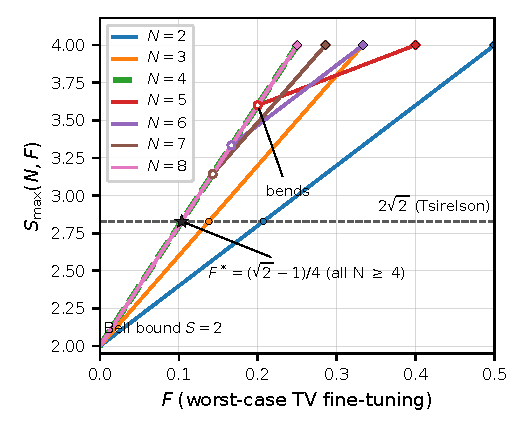
\includegraphics[width=\columnwidth]{fig_curves.pdf}
\caption{Exact curves $S_{\max}(N,F)$ for $N=2,\dots,8$ (Theorem~\ref{thm:curves}), computed in exact rational arithmetic from Eq.~\eqref{eq:thm1}. The $N=4$ and $N=8$ curves coincide ($2+8F$ up to $F=\tfrac14$, then $4$); the $N=4$ curve is drawn dashed so that both remain visible. Every curve starts at the Bell value $S=2$ with initial slope $2\min(N,4)$. Open circles mark the bends at $F=1/N$ for $N=5,6,7$, where rows of the maximizing multiset exhaust their wrong-sign states and the slope drops; diamonds mark the caps $F(S{=}4;N)=\lceil N/4\rceil/N$ (Eq.~\eqref{eq:cap}), beyond which each curve is flat at $S=4$. The star marks the saturation value $F^*=(\sqrt{2}-1)/4$, at which all curves with $N\ge4$ cross the Tsirelson value $2\sqrt{2}$ (dashed line); the dots are the $N=2,3$ crossings.}
\label{fig:curves}
\end{figure}

% =====================================================================
\section{The no-signalling sub-case}
\label{sec:ns}

\subsection{Definition and a gauge caveat}
We impose full no-signalling on the observed marginals: for every $a$,
$\sum_\lambda p[ab,\lambda]\,u[a,\lambda]$ is independent of $b$, and
symmetrically for Bob. A subtlety matters here: NS constrains single-party
marginals and is \emph{not} invariant under the per-state sign-flip gauge of
Theorem~\ref{thm:finitemax} --- the products $q_{ab}$ fix $S$ but not the marginals. The
witnesses below therefore specify full response tables $(u,v)$, not just
patterns; a naive ``patterns-only'' NS reduction fails.

\subsection{Two states: no violation at any fine-tuning level}
\label{sec:ns2}

\begin{theorem}
\label{thm:ns2}
Under full no-signalling, $S_{\mathrm{NS}}(2,F)=2$ for \emph{all}
$F\in[0,\tfrac12]$. No Bell violation is possible at any fine-tuning level
with two hidden states.
\end{theorem}

\begin{proof}[Proof (certificate)]
For $N=2$, each row is parameterised by the free variable
$t_{ab}=p[ab,\lambda_0]\in[\tfrac12-F,\tfrac12+F]$; $S$ is affine in the
four $t$'s. The mechanism behind the flatness is that full NS pins row
pairs on both sides at once: Alice's equations force $t_{a0}=t_{a1}$ whenever
$u[a,\cdot]$ is non-constant, and Bob's force $t_{0b}=t_{1b}$ whenever
$v[b,\cdot]$ is non-constant (e.g.\ $u[0,\cdot]\ne$ constant $\Rightarrow
t_{00}=t_{01}$). The four NS equations therefore collapse the four free
variables to a small number of independent groups, and $S$ is an affine
function of those groups over a box of half-width $F$. With only one side
constrained, half these pinning relations are absent and a slope-$4$
direction survives (the side finding below). Enumerating all
$2^8=256$ response vertices and closing under the four NS equations by
union-find reduces the free variables to groups; maximising the resulting
affine $S$ over the box gives, for each vertex, an explicit exact affine
function $A+BF$ (the sign of $B$ fixes which endpoint is maximal). The enumeration produces
$1312$ candidate affine functions $A+BF$ in total; every one satisfies
$A+BF\le2$ for all $F\in[0,\tfrac12]$ (checked at both endpoints), and
$S=2$ is attained for \emph{every} $F\in[0,\tfrac12]$ (e.g.\ the constant
responses $u\equiv v\equiv+1$, for which $E[ab]=1$ and hence $S=2$ at every
feasible row). Hence $S_{\mathrm{NS}}(2,F)\equiv2$. The certificate is exact (rational
arithmetic) and re-runnable; see Appendix~\ref{supp:verify}.
\end{proof}

\noindent
\emph{Side finding.} Under \emph{one-sided} NS only (Alice's marginals
independent of Bob's setting), the bound is not flat --- at $N=2$,
$S=2+4F$ is reachable; the flatness genuinely uses both sides. (This is a
constraint on the observed marginals; the different constraint that the
hidden source itself be independent of Bob's setting --- one-sided
\emph{measurement dependence} --- is treated separately in
Sec.~\ref{sec:onesided}.)

\subsection{All $N\ge3$: no-signalling is silent}
\label{sec:ns3}

\begin{theorem}[NS headline]
\label{thm:ns}
Under full no-signalling, for every $N\ge3$,
\begin{equation}
\begin{aligned}
F^*_{\mathrm{NS}}(N) &:= \min\{F:S_{\mathrm{NS}}(N,F)\ge 2\sqrt{2}\}\\
&= \frac{\sqrt{2}-1}{\min(N,4)} \;=\; F^*(N).
\end{aligned}
\label{eq:FstarNS}
\end{equation}
Fine-tuning to the CHSH Tsirelson value is completely NS-silent: the minimum
is identical with and without signalling, and it is attained by an explicit
no-signalling model at every $N\ge3$.
\end{theorem}

\begin{proof}
\emph{Lower bound.} NS restricts the feasible set, so
$S_{\mathrm{NS}}(N,F)\le S_{\max}(N,F)$. For $N\ge4$, Theorem~\ref{thm:global}
gives $S_{\max}\le 2+8F<2\sqrt{2}$ whenever $F<(\sqrt{2}-1)/4$; for $N=3$, the
exact curve of Theorem~\ref{thm:curves}, $S_{\max}(3,F)=2+6\min(F,\tfrac13)$,
gives $S_{\max}<2\sqrt{2}$ whenever $F<(\sqrt{2}-1)/3$. Hence
$S_{\mathrm{NS}}(N,F)<2\sqrt{2}$ for all $N\ge3$ with
$F<(\sqrt{2}-1)/\min(N,4)$.

\noindent
\emph{Upper bound --- explicit algebraic witnesses.}

\textbf{$N\ge4$.} Let $d=F^*=(\sqrt{2}-1)/4$. State $i=0,\dots,N-1$ lies in
class $j=i\bmod 4$, with class counts $n_j\in\{\lfloor N/4\rfloor,
\lceil N/4\rceil\}$. The construction is:
\begin{itemize}
\item \emph{Patterns:} state $i$ has miss-type $M_j$ (all four $C=+2$
patterns; Sec.~\ref{sec:model}).
\item \emph{Response gauge} (per class $j$):
\begin{equation}
\begin{aligned}
u[0,\cdot]&=(+,+,-,-), & u[1,\cdot]&=(-,+,+,-),\\
v[0,\cdot]&=(-,+,-,-), & v[1,\cdot]&=(+,-,-,-),
\end{aligned}
\label{eq:ns4gauge}
\end{equation}
i.e.\ the $j$-th entry of each tuple gives the response of states in class
$j$. One checks that the resulting per-state products are exactly
$M_A,M_B,M_C,M_D$ for classes $0,1,2,3$.
\item \emph{Rows:} $p[ab,i]=\frac1N+x[ab,\,i\bmod 4]$ with (all other
$x=0$)
\begin{equation}
\begin{array}{lll}
x[00,0]&=-d/n_0, & x[00,1]=+d/n_1,\\
x[01,0]=+d/n_0, & x[01,1]=-d/n_1,\\
x[10,1]=+d/n_1, & x[10,2]=-d/n_2,\\
x[11,0]=+d/n_0, & x[11,3]=-d/n_3.
\end{array}
\label{eq:ns4rows}
\end{equation}
\end{itemize}
Verification is exact (rational and $\mathbb{Q}(\sqrt2)$ arithmetic;
certificate in Appendix~\ref{supp:verify}):
\begin{itemize}
\item \emph{Rows.} $n_r\,x[ab,r]=-d$ and $\sum_{j\ne r}n_j x[ab,j]=+d$ hold
identically for each row, so every row has TV exactly $d$ and is bang--bang
in its $\sigma_{ab}$-direction. Feasibility $p\ge0$ requires
$d/n_r\le 1/N\iff n_r\ge dN$ for all $r$ --- precisely the case-checked
inequality $\lfloor N/4\rfloor\ge(\sqrt{2}-1)N/4$ of
Sec.~\ref{sec:headline}.
\item \emph{NS.} Each NS equation --- Alice's equating rows $a0$ and $a1$
(weighted by $u_a$), Bob's equating rows $0b$ and $1b$ (weighted by $v_b$) ---
reduces to $\sum_j n_j x[ab_L,j]\,w_j=\sum_j n_j x[ab_R,j]\,w_j$ for the
response values $w_j$ (the uniform parts cancel). Substituting
Eqs.~\eqref{eq:ns4gauge} and \eqref{eq:ns4rows}, each side is a sum of at
most two terms; all four close explicitly. Alice $a{=}0$ (rows $00$ vs $01$,
$u_0=(+,+,-,-)$): $\;n_0(-d/n_0)(+1)+n_1(d/n_1)(+1)=-d+d$ versus
$n_0(d/n_0)(+1)+n_1(-d/n_1)(+1)=d-d$. Alice $a{=}1$ (rows $10$ vs $11$,
$u_1=(-,+,+,-)$): $\;n_1(d/n_1)(+1)+n_2(-d/n_2)(+1)=d-d$ versus
$n_0(d/n_0)(-1)+n_3(-d/n_3)(-1)=-d+d$. Bob $b{=}0$ (rows $00$ vs $10$,
$v_0=(-,+,-,-)$): $\;n_0(-d/n_0)(-1)+n_1(d/n_1)(+1)=2d$ versus
$n_1(d/n_1)(+1)+n_2(-d/n_2)(-1)=2d$. Bob $b{=}1$ (rows $01$ vs $11$,
$v_1=(+,-,-,-)$): $\;n_0(d/n_0)(+1)+n_1(-d/n_1)(-1)=2d$ versus
$n_0(d/n_0)(+1)+n_3(-d/n_3)(-1)=2d$. Each identity is $0=0$ or $2d=2d$,
independent of the class counts $n_j$; the same closure was verified exactly
for all $N=4,\dots,64$.
\item \emph{Value.} Each row contributes $\mu_{ab}+2d$, so
$S=S_0+8d=2+8F^*=2\sqrt{2}$, with $\TV(p_{ab}\Vert\rho)=d$ for all $ab$ and
NS holding. Hence $F^*_{\mathrm{NS}}(N)\le F^*$ for all $N\ge4$.
\end{itemize}

\textbf{$N=3$.} In $\mathbb{Q}(\sqrt2)$, set $d_3=(\sqrt{2}-1)/3$; the
patterns are $\{M_A,M_B,M_D\}$ on states $1,2,3$, with response gauge
\begin{equation}
\begin{aligned}
u[0,\cdot]&=(-,-,+), & u[1,\cdot]&=(+,-,+),\\
v[0,\cdot]&=(+,-,+), & v[1,\cdot]&=(-,+,+),
\end{aligned}
\label{eq:ns3gauge}
\end{equation}
and rows (entries are $\frac13$ plus $d_3$ times the coefficient shown)
\begin{equation}
\begin{array}{c|ccc}
 & \lambda_1 & \lambda_2 & \lambda_3\\ \hline
00 & -1 & +\tfrac12 & +\tfrac12\\[2pt]
01 & +\tfrac12 & -1 & +\tfrac12\\[2pt]
10 & -\tfrac12 & +\tfrac12 & 0\\[2pt]
11 & +\tfrac12 & +\tfrac12 & -1
\end{array}
\label{eq:ns3rows}
\end{equation}
Exact $\mathbb{Q}(\sqrt2)$ arithmetic gives $S=2+6d_3=2\sqrt{2}$, per-row TV
$=(d_3,d_3,d_3/2,d_3)$, and all four NS residuals exactly zero. Hence
$F^*_{\mathrm{NS}}(3)\le d_3$. (The saved certified array --- available from
the authors, Appendix~\ref{supp:verify} --- differs from this printed gauge
by the global flip $(u,v)\mapsto(-u,-v)$, which leaves every product $q_{ab}$
--- hence $S$ --- and the setting-independence of each one-party marginal
unchanged.)

Lower and upper bounds together give Eq.~\eqref{eq:FstarNS} for all $N\ge3$,
with explicit algebraic witnesses at every $N$ --- an existence-free
statement.
\end{proof}

\noindent
\emph{Remark (the whole NS curve on $[0,F^*$].)} Every constraint of the
$N\ge4$ construction is linear in $d$, so scaling $d$ to any
$F\in[0,F^*]$ gives a valid NS model with $\TV(p_{ab}\Vert\rho)=F$ and
$S=2+8F$ (feasibility holds throughout). With the global upper bound
$S_{\mathrm{NS}}\le S_{\max}\le 2+8F$, this yields
\begin{equation}
S_{\mathrm{NS}}(N,F) = 2+8F \qquad\text{on }[0,F^*]\ \text{for all } N\ge4:
\label{eq:nscurve}
\end{equation}
the NS curve coincides with the signalling-allowed curve up to the quantum
point.

\subsection{The algebraic maximum under no-signalling}
\label{sec:ns4}

The silence of Sec.~\ref{sec:ns3} extends to the algebraic maximum $S=4$:
the unique NS box that reaches it is the PR box, and the minimum
fine-tuning of a local no-signalling decomposition of that box equals the
signalling-allowed cap.

\begin{lemma}[PR-box uniqueness]
\label{lem:pr}
A no-signalling CHSH box with $S=4$ is uniquely the
Popescu--Rohrlich (PR) box \cite{pr1994} (a standard fact, recorded here for completeness): at $(a,b)=(0,0),(0,1),(1,0)$ it outputs
$x=y$ with $P(+,+)=P(-,-)=1/2$, and at $(1,1)$ it outputs $x=-y$ with
$P(+,-)=P(-,+)=1/2$; all single-party marginals are uniform.
\end{lemma}

\begin{proof}
$S=E[00]+E[01]+E[10]-E[11]=4$ with $|E[ab]|\le1$ forces
$E[ab]=\sigma_{ab}$ at all four corners. Since $x,y\in\{\pm1\}$,
$E[ab]=+1$ means $x=y$ almost surely, and $E[11]=-1$ means
$x=-y$ almost surely. Write the NS marginals as
$\alpha_a=P(x{=}{+}1\mid a)$, $\beta_b=P(y{=}{+}1\mid b)$ (NS makes them
independent of the distant setting). The three $x=y$ corners give
$\alpha_0=\beta_0$, $\alpha_0=\beta_1$, $\alpha_1=\beta_0$; the $x=-y$
corner gives $\alpha_1=1-\beta_1$. The first three yield a common value
$r$; the last gives $r=1-r$, hence $r=1/2$, and the box is fully
determined.
\end{proof}

\noindent
\emph{Consequence.} A fine-tuned local deterministic model that is
no-signalling and reaches $S=4$ is \emph{exactly} a local decomposition of
the PR box:
$P(x,y\mid a,b)=\sum_\lambda p[ab,\lambda]\,
\mathbf{1}[x=u[a,\lambda]]\,\mathbf{1}[y=v[b,\lambda]]$ with per-row
$\TV(p(\cdot\mid ab)\Vert\rho)\le F$. The question is therefore: what is
the minimum TV cost of a local decomposition of the PR box, as a function
of the number $N$ of hidden states? (The PR box is NS but nonlocal --- it
has no such decomposition at $F=0$; the question is how much measurement
dependence must be imported to make it local.)

\begin{theorem}
\label{thm:ns4cap}
For every $N\ge3$,
\begin{equation}
F^*_{\mathrm{NS}}(S{=}4;N) := \min\{F : S_{\mathrm{NS}}(N,F)\ge 4\}
\;=\; \frac{\lceil N/4\rceil}{N}.
\label{eq:ns4cap}
\end{equation}
No-signalling neither raises nor lowers the signalling-allowed cap of
Theorem~\ref{thm:cap}. The case $N=2$ is excluded: by
Theorem~\ref{thm:ns2}, $S_{\mathrm{NS}}(2,F)=2$ for all $F$, so $S=4$ is
unattainable there at any fine-tuning level.
\end{theorem}

\begin{proof}
\emph{Lower bound.} NS restricts the feasible set, so
$S_{\mathrm{NS}}(N,F)\le S_{\max}(N,F)$ and hence
$F^*_{\mathrm{NS}}(S{=}4;N)\ge F(S{=}4;N)=\lceil N/4\rceil/N$ by
Theorem~\ref{thm:cap}; no NS-specific argument is needed, since the
parity-lemma necessity behind that cap ($S=4\Rightarrow E[ab]=\sigma_{ab}$
for all $ab$, so each row must be supported on its correct class, forcing
$F\ge n_{ab}/N$ with $\max_{ab}n_{ab}\ge\lceil N/4\rceil$) does not use NS.

\emph{Upper bound --- closed-form construction.} Use the round-robin
patterns of Sec.~\ref{sec:qN}: state $i$ carries miss-type
$M_{i\bmod 4}$, with class $j$ of size
$n_j\in\{\lfloor N/4\rfloor,\lceil N/4\rceil\}$. The response gauge is the
base realisation per type with one whole class flipped --- class $D$ if
$N\bmod 4\in\{0,1,2\}$, class $C$ if $N\bmod 4=3$ --- which leaves every
product $q_{ab}$ (hence the patterns and $S$) unchanged and only fixes the
NS marginals. Each row is then supported on its correct class $C_{ab}$ ---
the class that misses $ab$ carries mass $0$ --- so $E[ab]=\sigma_{ab}$ and
$S=4$. Writing $a,b,c,d=n_0,n_1,n_2,n_3$, the row masses on the four
classes are, in the flip-$D$ case,
\begin{equation}
\begin{array}{c|cccc}
 & A & B & C & D\\ \hline
00 & 0 & b/N & \tfrac12-b/N & \tfrac12\\
01 & b/N & 0 & \tfrac12-b/N & \tfrac12\\
10 & a/N & \tfrac12 & 0 & \tfrac12-a/N\\
11 & a/N & \tfrac12 & \tfrac12-a/N & 0
\end{array}
\label{eq:ns4caprows}
\end{equation}
(distributed uniformly within each class), and in the flip-$C$ case the
same display with $b$ replaced by $d$ and the roles of $C$ and $D$
swapped; all entries are non-negative for every $N\ge3$. Two facts close
the argument. \textbf{(NS automatic.)} Substituting the gauge into the
four NS residuals, each reduces to the difference of two identical sums
(e.g.\ Alice's $a{=}0$ residual is
$(b/N+(\tfrac12-b/N)-\tfrac12)-(b/N+(\tfrac12-b/N)-\tfrac12)$), so all
four vanish identically: no NS equation constrains the free entries beyond
the row sums. \textbf{(TV at or below the cap.)} Expanding the absolute
values, each per-row TV is the maximum of two branch values; in the
flip-$D$ case,
\begin{equation}
\begin{aligned}
\TV_{00} &= \max(a,\,N/2-d)/N,\\
\TV_{01} &= \max(b,\,N/2-d)/N,\\
\TV_{10} &= \max(N/2-b,\,c)/N,\\
\TV_{11} &= \max(N/2-b,\,d)/N.
\end{aligned}
\label{eq:ns4tv}
\end{equation}
Since every class count is $\le\lceil N/4\rceil$, it remains to check the
$N/2-(\mathrm{class})$ branches: for $N=4k+r$, $r\in\{0,1,2\}$, each is
$\le k+1=\lceil N/4\rceil$ (equality at $r=0,2$), and in the flip-$C$ case
($N=4k+3$) all four rows land at exactly $\TV=(k+1)/N
=\lceil N/4\rceil/N$. Hence $\TV(p(\cdot\mid ab)\Vert\rho)
\le\lceil N/4\rceil/N$ for all $ab$ and all $N\ge3$.
\end{proof}

\noindent
\emph{Explicit witnesses} (exact; certificate in Appendix~\ref{supp:verify}). At $N=3$ (class sizes $1,1,1,0$, flip $C$), the per-state rows
are $p[00,\cdot]=(0,\tfrac12,\tfrac12)$,
$p[01,\cdot]=(\tfrac12,0,\tfrac12)$,
$p[10,\cdot]=p[11,\cdot]=(\tfrac12,\tfrac12,0)$: $S=4$, per-row TV
$1/3$, all four NS residuals zero, so
$F^*_{\mathrm{NS}}(S{=}4;3)=\tfrac13$. At $N=4$ (class sizes $1,1,1,1$,
flip $D$), the per-state rows are
$p[00,\cdot]=(0,\tfrac14,\tfrac14,\tfrac12)$,
$p[01,\cdot]=(\tfrac14,0,\tfrac14,\tfrac12)$,
$p[10,\cdot]=(\tfrac14,\tfrac12,0,\tfrac14)$,
$p[11,\cdot]=(\tfrac14,\tfrac12,\tfrac14,0)$: $S=4$, per-row TV $1/4$,
NS residuals zero --- an explicit local decomposition of the PR box at
cost $1/4$, so $F^*_{\mathrm{NS}}(S{=}4;4)=\tfrac14$. At $N=5$ (class
sizes $2,1,1,1$, flip $D$), the class-mass rows are
$p[00,\cdot]=(0,\tfrac15,\tfrac{3}{10},\tfrac12)$,
$p[01,\cdot]=(\tfrac15,0,\tfrac{3}{10},\tfrac12)$,
$p[10,\cdot]=(\tfrac25,\tfrac12,0,\tfrac{1}{10})$,
$p[11,\cdot]=(\tfrac25,\tfrac12,\tfrac{1}{10},0)$: $S=4$, per-row TV
$\le\tfrac25$, NS residuals zero, so
$F^*_{\mathrm{NS}}(S{=}4;5)=\tfrac25$.

Hiding the fine-tuning from the marginals never raises the price of
reaching the algebraic maximum: no-signalling is silent at $S=4$ as well
as at $S=2\sqrt2$, and the cost is the same cap
$\lceil N/4\rceil/N$ as with signalling allowed.

% =====================================================================
\section{Explicit witness at the Tsirelson point}
\label{sec:witness}

The $N=4$ optimal point of the signalling-allowed problem, verified by direct
arithmetic and as an exact identity in $\mathbb{Q}(\sqrt2)$ (Appendix~\ref{supp:verify}), is: with
\begin{equation}
\begin{aligned}
F^*&=\frac{\sqrt2-1}{4}\approx0.1035534,\\
a&=\tfrac14-F^*\approx0.1464466, & b&=\tfrac14+F^*\approx0.3535534,
\end{aligned}
\label{eq:witconst}
\end{equation}
the conditional sources $p[ab,\lambda]$ (rows $=ab$ in order $00,01,10,11$;
columns $=\lambda=1,\dots,4$) are
\begin{equation}
\begin{array}{c|cccc}
 & \lambda_1 & \lambda_2 & \lambda_3 & \lambda_4\\ \hline
00 & \tfrac14 & a & b & \tfrac14\\
01 & a & \tfrac14 & b & \tfrac14\\
10 & b & \tfrac14 & a & \tfrac14\\
11 & b & \tfrac14 & \tfrac14 & a
\end{array}
\label{eq:witp}
\end{equation}
with deterministic responses
\begin{equation}
\begin{aligned}
u[0,\cdot]&=(+,-,-,-), & u[1,\cdot]&=(+,+,+,-),\\
v[0,\cdot]&=(+,+,-,-), & v[1,\cdot]&=(-,-,-,-).
\end{aligned}
\label{eq:wituv}
\end{equation}
Direct recomputation (independent of any optimisation) gives
$S=E[00]+E[01]+E[10]-E[11]=2\sqrt2$ and
$F=\max_{ab}\tfrac12\sum_\lambda|p[ab,\lambda]-\tfrac14|=(\sqrt2-1)/4$
exactly. A local, deterministic, finite model with a \emph{uniform} source
and only $\approx10.4\%$ settings-conditioned fine-tuning (TV) thus reaches
the maximal quantum CHSH violation exactly. (This is the signalling-allowed
witness; the no-signalling witness of Theorem~\ref{thm:ns} has a different
gauge and rows, since NS is not gauge-invariant.)

% =====================================================================
\section{Discussion}
\label{sec:discussion}

\subsection{Interpretation}
The fine-tuning cost decreases with $N$ but \emph{saturates at $N=4$}: adding
hidden states beyond four does not lower the minimum fine-tuning needed to
reach $2\sqrt2$. The bottleneck is the \emph{four CHSH correlators}, not the
size of the hidden source --- a four-state source already spends its budget
optimally across the four $(a,b)$ blocks, and more states just dilute without
reducing the per-correlator cost. (The qualitative observation that enlarging
the hidden-variable space does not reduce the required relaxation was made
earlier for mutual-information-metric singlet models \cite{rossisouza2018};
our saturation is its exact closed-form counterpart in a different metric and
target.) By Proposition~\ref{prop:general} the floor
$F^*\ge(\sqrt2-1)/4\approx0.1036$ is model-independent: \emph{any} local CHSH
model, on any hidden-variable space, with any source distribution and
deterministic or stochastic responses, that reaches the maximal quantum
violation must fine-tune at least one conditional source by at least
$(\sqrt2-1)/4\approx10.4\%$ in TV in its worst settings block.

The no-signalling results sharpen the picture further. The minimum
fine-tuning for $S=2\sqrt2$ is achievable \emph{without observable
signalling} for every $N\ge3$ (Theorem~\ref{thm:ns}), and the whole curve up
to the quantum point coincides with the signalling-allowed one
(Eq.~\eqref{eq:nscurve} for $N\ge4$; at $N=3$ the common curve is $2+6F$,
by the same scaling argument). The cost of measurement dependence is therefore
not paid in observable marginals: a local model can hide its
settings-dependence from the single-party statistics and still violate CHSH
maximally quantumly, at the same $\approx10.4\%$ price. This directly
addresses the claim of Bacciagaluppi \emph{et al.} that some
measurement-independence violations are ``signalling in principle''
\cite{bhl2026}: in this TV metric, the \emph{minimal} fine-tuning for a
maximal quantum CHSH violation is NS-silent (for $N\ge3$). Our statement
concerns observable marginals within a fixed model class; it neither refutes
nor settles the causal-structure notion of ``signalling in principle'' of
Ref.~\onlinecite{bhl2026}, which is a different question. The two-state case
is the converse: under full NS, no fine-tuning at all can produce a Bell
violation (Theorem~\ref{thm:ns2}) --- with two states, hiding the
fine-tuning from the marginals makes it useless.

\subsection{One-sided measurement dependence}
\label{sec:onesided}

A natural structural restriction, studied by Hall and Branciard in their
mutual-information programme \cite{hallbranciard2020}, is the
\emph{one-sided} causal structure: the hidden source depends on exactly one
setting, $p[ab,\lambda]=q[a,\lambda]$ (independent of $b$), with cost
$F_{\mathrm{os}}=\max_a\TV(q(a)\Vert\rho)$; by the $a\leftrightarrow b$
symmetry of CHSH, the Bob-only variant has identical values throughout.
Rows then come in pairs, $p[00]=p[01]=q_0$, $p[10]=p[11]=q_1$, and
\begin{equation}
\begin{aligned}
S &= \sum_\lambda q_0(\lambda)\,f^A(\lambda)
+\sum_\lambda q_1(\lambda)\,f^B(\lambda),\\
f^A(\lambda) &= q_{00}(\lambda)+q_{01}(\lambda),\\
f^B(\lambda) &= q_{10}(\lambda)-q_{11}(\lambda).
\end{aligned}
\label{eq:osrows}
\end{equation}
each $f^A,f^B$ taking values in $\{-2,0,+2\}$. The key structural fact: for
every even-parity pattern, \emph{exactly one} of $f^A(\lambda),f^B(\lambda)$
is non-zero --- each hidden state can actively bend only \emph{one} of the
two source rows. That single fact halves the slope of the loophole and
removes the saturation phenomenon.

\begin{lemma}[one-sided row optimum]
\label{lem:osrow}
Let $f\in\{-2,0,+2\}^N$ have $k$ entries equal to $+2$, $z$ entries equal
to $0$, and $m$ entries equal to $-2$, and set $\mu=2(k-m)/N$. Then
\begin{equation}
\begin{aligned}
h(f,F) &:= \max\bigl\{p\cdot f:\ p\in\Delta_N,\ \TV(p\Vert\rho)\le F\bigr\}\\
&\le\ \mu + 2F + 2\min(F,\,m/N)\;\le\;\mu+4F,
\end{aligned}
\label{eq:osrow}
\end{equation}
with the exact value a piecewise-linear function of $F$ (water-filling over
the three rate classes $+2,0,-2$) given in Appendix~\ref{supp:osdetails}.
\end{lemma}

\begin{proposition}
\label{prop:onesided}
For every $N\ge2$,
\begin{equation}
\begin{aligned}
F^*_{\mathrm{os}}(N) &:= \min\{F : S_{\mathrm{os}}(N,F)\ge 2\sqrt2\}\\
&= \frac{\sqrt2-1}{2}\;\approx 0.20711,
\end{aligned}
\label{eq:Fos}
\end{equation}
flat in $N$ from the start, and the one-sided global bound
$S_{\mathrm{os}}(N,F)\le 2+4F$ holds for all $N$ and all $F$.
\end{proposition}

\begin{proof}[Proof sketch]
\emph{Lower bound.} Fix the responses and let $k_A,m_A$ (resp.\ $k_B,m_B$)
count the entries of $f^A$ (resp.\ $f^B$) equal to $\pm2$. By the key
structural fact, $k_A+m_A+k_B+m_B=N$. Lemma~\ref{lem:osrow} bounds each row,
and a four-case analysis of whether the two row bounds are above or below
$2$ --- using $\mu_A+\mu_B=2-4(m_A+m_B)/N$, which forces the intercept down
whenever both rows are active --- gives
$S_{\mathrm{os}}(N,F)\le 2+4F$ for all $N,F$ (exact case analysis in Appendix~\ref{supp:osdetails}). Hence $S_{\mathrm{os}}(N,F)<2\sqrt2$ for
$F<(\sqrt2-1)/2$.
\emph{Upper bound.} Take $\lceil N/2\rceil$ states of a pattern with
$f^A=+2$ and $\lfloor N/2\rfloor$ states of one with $f^B=+2$; then row $A$
has $(k,m,z)=(\lceil N/2\rceil,0,\lfloor N/2\rfloor)$ and row $B$ the
mirror, both in the slope-2 regime of Lemma~\ref{lem:osrow}, so
$S_{\mathrm{os}}(N,F)\ge 2+4\min(F,\lfloor N/2\rfloor/N)$. Since
$(\sqrt2-1)/2<\lfloor N/2\rfloor/N$ for all $N\ge2$ (an exact
$\mathbb{Q}(\sqrt2)$ identity, checked in the certificate), the
construction reaches $S=2+4F_{\mathrm{os}}=2\sqrt2$ at
$F_{\mathrm{os}}=(\sqrt2-1)/2$.
\end{proof}

\noindent
\emph{Consequences.} The one-sided cost equals the full-structure value at
$N=2$ exactly: adding hidden states never helps, so in cost terms the
one-sided structure is worth throwing away every state beyond two. The
penalty factor relative to the full causal structure is \emph{exactly
$2$} for $N\ge4$ (and $3/2$ at $N=3$), since
$F^*_{\mathrm{os}}(N)/F^*(N)=\min(N,4)/2$. The cap to $S=4$ under
one-sided dependence is $\lceil N/2\rceil/N$ (proved): exactly twice the
full-model cap $\lceil N/4\rceil/N$ for $N\equiv 0,3\ (\mathrm{mod}\,4)$,
and a factor $\ge\tfrac32$ (tending to $2$) for $N\equiv 1,2\
(\mathrm{mod}\,4)$ with $N\ge5$ (at $N=2$ the two caps coincide, both
equal to $\tfrac12$). Hall and Branciard's mutual-information metric gives
the same qualitative ordering --- one-sided $\approx0.128$ bits versus
causal $\approx0.080$ bits, a factor $\approx1.6$ --- whereas the TV metric
gives the factor exactly $2$; the two metrics are incommensurable, so no
cross-metric ordering of the absolute numbers follows (Sec.~\ref{sec:metric}).
The exact one-sided curves $S_{\mathrm{os},\max}(N,F)$ for
$N=2,\dots,8$ are certified in Appendix~\ref{supp:osdetails}: for even $N$ the
curve is the single segment $\min(2+4F,4)$ (proved for \emph{all} even
$N$), and for odd $N$ it bends once at $F=\lfloor N/2\rfloor/N$ (proved for
$N=3,5,7$; the bend line for odd $N\ge9$ is conjectured).

\subsection{Relation to prior work}
\label{sec:related}

Table~\ref{tab:lit} positions this work relative to the closest prior
literature (all entries independently verified against arXiv; a completed
2015--2026 sweep with full search log is described in Appendix~\ref{supp:sweep}).

\begin{table}[!htbp]
\caption{Comparison of fine-tuning metrics and values at the CHSH Tsirelson
point $S=2\sqrt2$. ``Ret.'' = fraction of independence retained.}
\label{tab:lit}
\small
\begin{tabular}{@{}>{\raggedright\arraybackslash}p{2.6cm}>{\raggedright\arraybackslash}p{2.9cm}>{\raggedright\arraybackslash}p{2.8cm}@{}}
\toprule
Work & Metric & Value at $S=2\sqrt2$ \\ \midrule
Hall \cite{hall2010}
& pairwise $L^1$ distance $M\in[0,2]$ between setting-pair sources; NS, continuous $\lambda$
& $M_{\mathrm{singlet}}=\tfrac{2}{3}(\sqrt2-1)\approx0.276$ (ret.\ $\approx0.862$) \\ \addlinespace
Hall \& Branciard \cite{hallbranciard2020}
& mutual information $I(X,Y:\Lambda)$ in bits, fixed causal structures
& causal $\approx0.080$; retrocausal $\approx0.046$; one-sided $\approx0.128$; superdet $=2$ bits \\ \addlinespace
Friedman \emph{et al.} \cite{fghk2019}
& per-observer Hall-type parameters, combined relaxations
& tight general bounds (no single number) \\ \addlinespace
Takakura \emph{et al.} \cite{takakura2022}
& Hall's $M$ + hidden information $H=1-\max_\lambda p(\lambda)$
& $S\le 2+\min\{3M,\tfrac34 M+2H,2\}$, necessary \& sufficient \\ \addlinespace
Pal \emph{et al.} \cite{pal2026}
& ensemble-divergence $\delta_{\mathrm{ens}}$ (TV-type) for drifting preparations; MI preserved
& $|S|\le 2+6\delta_{\mathrm{ens}}$ (not claimed tight) \\ \addlinespace
Alai \cite{alai2026a}
& Hall-type variational $M$ (normalised as Hall's $M/2$) + detector efficiency $\eta_{\mathrm{eff}}$
& closed form $M(S,\eta)$; at $\eta=1$: $(\sqrt2-1)/3\approx0.1381$ \\ \addlinespace
Alai \cite{alai2026b}
& Hall's $M$, $F:=M/2$ (GHZ--Mermin)
& $F(n)=R/[2(R+1)]$ ($R=2^{\lfloor(n-1)/2\rfloor}$) for $n=3,\dots,13$; CHSH consistency value $(\sqrt2-1)/3$ \\ \addlinespace
\textbf{This work}
& per-setting $\TV(p(\cdot|ab)\Vert\rho)$ from a fixed baseline source
& $F^*=(\sqrt2-1)/\min(N,4)\approx0.1036$ ($N\ge4$), exact; NS-silent for $N\ge3$ \\ \bottomrule
\end{tabular}
\end{table}

\emph{Three similar numbers --- disambiguation.} (i) Hall's $L^1$ convention:
$M_{\mathrm{singlet}}=\tfrac23(\sqrt2-1)\approx\mathbf{0.276}$.
(ii) Fraction-of-independence-lost convention ($M/2$):
$(\sqrt2-1)/3\approx\mathbf{0.1381}$ --- Hall's $S=2\sqrt2$ cost in that
convention, and the $\eta=1$ floor of Ref.~\onlinecite{alai2026a}.
(iii) Our per-block TV metric: $F^*=(\sqrt2-1)/4\approx\mathbf{0.1036}$.
These come from different metrics on different model classes; no ordering of
the numbers follows, and none contradicts any other. Hall's metric is
pairwise (no fixed baseline) and his bound is derived for no-signalling
models; ours measures each conditional source $p(\cdot\mid ab)$ against a
fixed uniform baseline and allows (optionally forbids) signalling. Our TV is a different,
non-information-theoretic measure of the same statistical-independence
violation; explicit conversion bounds between the conventions for the
\emph{same} model, and the identification of our model class with the
general (retrocausal) causal structure of
Ref.~\onlinecite{hallbranciard2020}, are worked out in
Sec.~\ref{sec:metric}.

\emph{Relation to the MDL--CHSH bound of P\"utz \emph{et al.}} The
closest prior result is not in a Hall-type metric at all. P\"utz
\emph{et al.} \cite{putz2014,putzgisin2016} parametrise measurement
dependence by bounds $\ell\le P(x,y\mid\lambda)\le h$ on the settings given
the hidden variable, and show that measurement-dependent local
correlations with no-signalling and uniform inputs reach at most
$\mathrm{CHSH}=4(1-2\ell)$ (their Eq.~(11), resp.\ Eq.~(31)), so that
quantum theory can violate the bound only for $\ell>(2-\sqrt2)/4$. Their
extremal construction distributes the four single-miss strategies, each
keeping probability $\ell$ on its one wrong input pair and $(1-\ell)/3$ on
the other three; read in our variables (uniform inputs, $\rho=1/4$) this is
exactly the round-robin $N=4$ model with every row at total-variation
distance $\tfrac14-\ell$ from uniform. Substituting $\ell=\tfrac14-F$ turns
$4(1-2\ell)$ into $2+8F$ and $(2-\sqrt2)/4$ into $(\sqrt2-1)/4$: the
four-state headline of this paper --- the linear law and the Tsirelson
threshold --- is a re-parametrisation of their result, reached here by a
different route (a per-row TV lemma rather than vertex enumeration of the
MDL polytope). The two metrics are nevertheless not equivalent in general:
$\ell$ bounds the ratio $p(\lambda\mid x,y)/\bar\rho(\lambda)$ from below,
$F$ bounds an $L^1$ distance, and a model can sit at different points in
the two variables (the NS witness of Theorem~\ref{thm:ns} has
$\ell=(\tfrac14-d)/(1+d)\ne\tfrac14-d$). What Refs.~\onlinecite{putz2014,
putzgisin2016} do not contain, and this paper adds, is the TV bound for
arbitrary source distributions and hidden-variable spaces
(Proposition~\ref{prop:general}), the exact finite-$N$ curves and caps,
the two-state no-signalling impossibility, the no-signalling cap at $S=4$,
the one-sided value, and the conversions to Hall's $M$ and to mutual
information. More broadly, how much measurement dependence is ``enough''
depends on both the metric and the target correlations: in the
$\ell$-parametrisation any nonzero residual independence can be detected
by suitable quantum correlations \cite{putz2014}, whereas in Hall's $M$
\cite{hall2010}, in mutual information \cite{barrettgisin2011,
hallbranciard2020} and in our TV metric a fixed modest amount reproduces
the CHSH Tsirelson value. Our result is one exactly solved point in that
landscape, not a metric-independent price of the loophole.

\emph{Novelty, stated as a search result.} Within arXiv-indexed literature
through 2026-09-02, no prior use was found of (i) the per-setting
TV-from-a-fixed-source metric, (ii) the exact closed forms
$F^*=(\sqrt2-1)/\min(N,4)$ with $N=4$ saturation together with the exact
curves and cap $\lceil N/4\rceil/N$ --- with the important qualification,
found in review, that the $N=4$ value is equivalent to the MDL--CHSH
threshold of P\"utz \emph{et al.} discussed above --- or (iii) an
NS-silence result of this kind. This is stated as a search result, not ``proven novel'': coverage was
arXiv-centric ($\sim$16 papers read at full or abstract depth, the rest at
catalogue level); paywalled journal content not mirrored on arXiv, non-arXiv
repositories, and books/theses are not covered. The closest prior work is
Ref.~\onlinecite{alai2026a} --- exact minimum measurement dependence for CHSH
via LP (machine precision on a 32-point grid, with an exact
$\mathbb{Q}(\sqrt2)$ certificate at one point), in a Hall-type metric
normalised as Hall's $M/2$, plus detector-efficiency degrees of freedom; its $\eta=1$ floor at $2\sqrt2$,
$(\sqrt2-1)/3\approx0.1381$, is a different number from our
$F^*=(\sqrt2-1)/4\approx0.1036$ because the metrics differ --- no
contradiction. Together with Refs.~\onlinecite{alai2026b,pal2026,takakura2022},
this shows that ``exact minimum measurement dependence'' is an active 2026
front; our contribution is a specific metric with clean closed forms, plus
the NS sub-case, which none of them covers.

\subsection{Implications for proposed superdeterministic models}
\label{sec:superdet}

The model-independence of Proposition~\ref{prop:general} means that the
floor $F^*\ge(\sqrt2-1)/4\approx10.4\%$ is a price attached to the
\emph{statistics} of any local account of the Tsirelson value, independent
of the causal story told for the settings-dependence. Several explicit
models have been proposed in the superdeterminism literature, and all fall
on the priced side of this bound. Brans's fully causal model
\cite{brans1988} --- in which the hidden variable determines both outcomes
and settings and reproduces the singlet correlations for arbitrary spin-1/2
directions, as described in Ref.~\onlinecite{hall2010} --- is a direct
instance of our model class with a settings-dependent conditional source
$p(\lambda\mid a,b)$; if it reaches $S=2\sqrt2$, some settings block must
carry $\ge10.4\%$ TV. 't~Hooft's program of classical deterministic underpinnings
\cite{tHooft2021} claims that any quantum model can be mimicked to
arbitrary finite accuracy by classical deterministic dynamics, with Bell's
theorem inapplicable because the realistic state distribution depends on
the measurement basis; reaching $S=2\sqrt2-\varepsilon$ in such a
construction forces $F\ge(\sqrt2-1)/4-O(\varepsilon)$. In Palmer's
discretised Hilbert-space models \cite{palmer2022,palmer2024} the hidden
variable determines the actual apparatus settings, so conditioning on
observed settings restricts $\lambda$ to a proper subset of its domain;
since total variation is non-increasing under coarse-graining, any level of
description that locally reproduces $2\sqrt2$ forces $F\ge10.4\%$ at the
fine-grained level as well --- ``invisible to coarse-graining'' arguments
cannot lower the cost below the floor. (Palmer's separate claim that his
framework is not fine-tuned with respect to a $p$-adic metric on its state
space concerns a different metric and is not addressed by our bound.) The
most explicit recent
construction we examined, Garza and Hance's conservation-law model
\cite{garzahance2025}, keeps a fixed uniform baseline source while
measurement error removes a settings-dependent band from the
hidden-variable domain; at its best-fit parameter it reaches
$|S|\approx2.826$, within $0.08\%$ of the Tsirelson value, with
worst-block TV of $\approx17$--$29\%$ --- a factor $\approx1.7$--$2.8$
above the floor --- and the inequality $S\le2+8F$ holds across its
parameter space (verified numerically; Appendix~\ref{supp:verify}).
\footnote{The lower end of the range, $\approx17\%$, comes from a
two-band mixture that is \emph{our} reconstruction of their
single-$\lambda$ formulation; under the literal per-band reading the
worst-block TV is $s/\pi\approx29.2\%$. We report the range and flag the
$\approx1.7\times$ spread as reading-dependent. These figures are
floating-point evaluations of the authors' published formulas, not
exact-arithmetic certificates.}
We also note a point of self-consistency in that construction: their
correlator (their Eq.~(14)) satisfies $|E(\theta;\Delta L)|\le1$ for all
$\theta$ if and only if $\Delta L\ge\tfrac12$, and their model already
takes $\Delta L\ge0.5$ --- nothing they claim lies in the $|E|>1$ regime.
We stress what the bound does and does not say: it is compatible with every
one of these models, and it rules out none of them; it fixes a
quantitative price floor for the loophole, so that ``a little
fine-tuning'' in the sense of $<10.4\%$ TV per settings block is
insufficient, by theorem, for any local reproduction of the maximal
quantum violation. Whether such a deviation is physically plausible is a
separate question. Experimental model selection weighs against
superdeterministic causal structures \cite{daley2022}, and Vieira,
Ramanathan and Cabello have shown theoretically that local models with
\emph{partially} relaxed measurement independence (and parameter
independence) can be excluded by Bell-like experiments with many settings on
high-dimensional entangled states \cite{vieira2025}; that exclusion does not
cover the two-setting CHSH scenario priced here, but it delimits how far the
loophole can be pushed.

\subsection{Metric comparison}
\label{sec:metric}

The fine-tuning cost can be measured in four conventions
(Table~\ref{tab:metrics}). They all measure the same
statistical-independence violation and differ only in (i) whether a fixed
baseline $\rho$ is used and (ii) the $L^1$-vs-half-$L^1$-vs-entropy
functional --- which is exactly why explicit conversion bounds exist
between them.

\begin{table}[htbp]
\caption{The fine-tuning conventions of this work and the closest
literature. $p_{ab}=p(\cdot\mid a,b)$,
$\TV(p\Vert q)=\tfrac12\|p-q\|_1$, $p_{\mathrm{avg}}=\tfrac14\sum_{ab}p_{ab}$.}
\label{tab:metrics}
\small
\begin{tabular}{@{}>{\raggedright\arraybackslash}p{3.1cm}>{\raggedright\arraybackslash}p{5.3cm}@{}}
\toprule
Metric & Definition \\ \midrule
$F$ (this work)
& $\max_{ab}\TV(p_{ab}\Vert\rho)$: worst case from a \emph{fixed} baseline $\rho$ \\ \addlinespace
$M_{\mathrm{model}}$
& $\max_{ab,a'b'}\TV(p_{ab}\Vert p_{a'b'})$: pairwise, no baseline \\ \addlinespace
$M$ (Hall \cite{hall2010})
& $\max_{ab,a'b'}\|p_{ab}-p_{a'b'}\|_1 = 2M_{\mathrm{model}}$ \\ \addlinespace
$I(X,Y;\Lambda)$ (H\&B \cite{hallbranciard2020})
& $H(\Lambda)-\tfrac14\sum_{ab}H(\Lambda\mid a,b)$, in bits (equal to their $I(X,Y{:}\Lambda)$ for uniformly distributed settings, as they assume) \\ \bottomrule
\end{tabular}
\end{table}

\emph{Conversion bounds.} For every local CHSH model and every baseline
$\rho$:
\begin{enumerate}
\item $M_{\mathrm{model}}\le 2F$, by the triangle inequality,
$\TV(p_{ab}\Vert p_{a'b'})\le\TV(p_{ab}\Vert\rho)
+\TV(p_{a'b'}\Vert\rho)\le 2F$;
\item $F\le M_{\mathrm{model}}+\TV(p_{\mathrm{avg}}\Vert\rho)$, by
$\TV(p_{ab}\Vert\rho)\le\TV(p_{ab}\Vert p_{\mathrm{avg}})
+\TV(p_{\mathrm{avg}}\Vert\rho)$ and taking the maximum over $ab$;
\item no bound $F\le f(M_{\mathrm{model}})$ holds for a \emph{fixed}
external $\rho$: if all four rows equal some $q\ne\rho$, then
$M_{\mathrm{model}}=0$ while $F=\TV(q\Vert\rho)>0$.
\end{enumerate}
Bound~(i) is tight: for both $N=4$ witnesses
(Secs.~\ref{sec:ns} and \ref{sec:witness}) the six pairwise TVs take
values in $\{\delta,2\delta\}$ with $\delta=F^*$, so
$M_{\mathrm{model}}=2F^*$ exactly --- but it is not saturated by every
$F^*$-optimal witness: the $N=3$ NS witness of
Theorem~\ref{thm:ns} has $M_{\mathrm{model}}=\tfrac32F^*$ (slack
$F^*/2$).

\emph{Our witnesses in the other conventions.} The $F^*$-optimal $N=4$
witnesses cost $M_{\mathrm{model}}=2F^*=(\sqrt2-1)/2\approx0.207$ in the
pairwise-TV convention, i.e.\ Hall's full-$L^1$ value
$M=\sqrt2-1\approx0.414$ --- which in his ``fraction of independence
retained'' reads $1-M/2=(3-\sqrt2)/2\approx0.793$ --- and they carry
$I(X,Y;\Lambda)\approx0.056$ bits; the $N=3$ NS witness carries
$\approx0.055$ bits.

\emph{Different metrics select different optima.} Our TV-optimal witness is
not $M$-optimal: Hall's bound $S\le\min\{2+3M,4\}$ --- stated by Hall for deterministic
no-signalling models; we re-prove it in Appendix~\ref{supp:verify} using only
local determinism --- at $M=\sqrt2-1$ allows up to
$S=3\sqrt2-1\approx3.24$, whereas our witness sits at
$2\sqrt2\approx2.83$; nor is it MI-optimal, its $\approx0.056$ bits
exceeding the relevant floor of $\approx0.046$ bits. Different metrics
select different optimal models; this is why the three numbers of the
disambiguation above ($0.276/0.138/0.104$) coexist without
contradiction.

\emph{Model-class identification.} Ref.~\onlinecite{hallbranciard2020}
minimizes $I(X,Y;\Lambda)$ under fixed causal graphs. Its causal structure
imposes the additional factorization constraint that the two
\emph{settings} be conditionally independent given the hidden variable,
$p(a,b\mid\lambda)=p(a\mid\lambda)\,p(b\mid\lambda)$ (written
$p(x,y\mid\lambda)=p(x\mid\lambda)p(y\mid\lambda)$ in
Ref.~\onlinecite{hallbranciard2020}, whose $x,y$ denote settings), which our
closed-form witnesses do \emph{not} satisfy (verified exactly in
$\mathbb{Q}(\sqrt2)$ for every witness of this paper); equivalently, since
Ref.~\onlinecite{hallbranciard2020} proves its causal floor
$\approx0.080$ bits is the minimum over that class, no causal model can
reach $2\sqrt2$ at $\approx0.056$ bits. Our model class --- free
$p(\lambda\mid a,b)$ against a fixed $\rho$ --- is therefore H\&B's
\emph{general} (retrocausal) structure, for which the relevant floor at
$S=2\sqrt2$ is $I_{\mathrm{R}}\approx0.046$ bits, not the causal floor
$I_{\mathrm{C}}\approx0.080$; our witnesses' $\approx0.056$ bits sit above
it, as they must.

\emph{A sharper bound in our variable.} Hall's $S\le2+3M$ becomes
$S\le2+12F$ when written in our variable ($M=2M_{\mathrm{model}}\le4F$),
versus our direct $S\le2+8F$: TV from a fixed $\rho$ yields the sharper
CHSH bound because all four rows share one center.

\begin{proposition}[aggregation robustness]
\label{prop:avg}
(i) For every local CHSH model --- any source, deterministic or
stochastic responses --- $S\le2+8F_{\mathrm{avg}}$, where
$F_{\mathrm{avg}}=\tfrac14\sum_{ab}\TV(p(\cdot\mid ab)\Vert\rho)$.
(ii) The $N=4$ witness of Sec.~\ref{sec:witness} has all four per-row TVs
equal to $d=(\sqrt2-1)/4$, so
$F^*_{\mathrm{avg}}(4):=\min\{F_{\mathrm{avg}}:S=2\sqrt2\text{ achievable}\}
=d=F^*(4)$.
\end{proposition}

\begin{proof}[Proof sketch]
(i) The per-row estimate
$|\sigma_{ab}E[ab]-\mu_{ab}|\le2\TV(p(\cdot\mid ab)\Vert\rho)$ behind
Proposition~\ref{prop:general} uses only the \emph{row's own} TV; summing
the four rows with row-specific TVs gives
$S\le S_0+2\sum_{ab}\TV(p(\cdot\mid ab)\Vert\rho)=S_0+8F_{\mathrm{avg}}
\le2+8F_{\mathrm{avg}}$. (ii) An exact $\mathbb{Q}(\sqrt2)$ certificate
(Appendix~\ref{supp:verify}) re-derives the witness arithmetic: the four
per-row TVs are all exactly $d$, so its average-TV cost is $d$, and (i)
gives the reverse inequality.
\end{proof}

\noindent
The headline is therefore insensitive to the aggregation choice at $N=4$:
fine-tuning cannot be made cheaper by spreading it across the setting
blocks rather than concentrating it in one. What is \emph{not} claimed:
$F^*_{\mathrm{avg}}(N)$ for $N>4$ has not been computed; only the
model-independent floor $(\sqrt2-1)/4$ and the $N=4$ equality are proved.

\subsection{Scope, caveats, and verification}
The exact \emph{curves} are certified for $N=2,\dots,14$ (exhaustive
enumeration; Theorem~\ref{thm:curves} prints $N\le8$); for $N\ge15$ the first
segment, the cap, and the headline $F^*$ are proved for all $N$, while the
full bend region is left to numerics. The
exact finite-$N$ statements are certified for the \emph{uniform} source;
Proposition~\ref{prop:general} shows the lower bound
$F^*\ge(\sqrt2-1)/4$ does not depend on the source distribution or on
determinism, so no extension can lower the floor. Finally, $F^*$ is a
mathematical minimum within the model class --- it is not compared to any
physical prior on how much fine-tuning a real source could have.

Every result in this paper is checkable without trusting the prose: the exact
statements carry re-runnable exact-arithmetic certificates (rational and
$\mathbb{Q}(\sqrt2)$, no floating point; exit code $0$ iff every assertion
passes), and an independent LP pipeline reproduces the same values to
$\le1.8\times10^{-15}$. The full verification record, including how to re-run
each check, is in Appendix~\ref{supp:verify}.

% =====================================================================
\section{Conclusion}
\label{sec:conclusion}

We quantified the price of the measurement-dependence escape route for
Bell/CHSH in a per-setting total-variation metric and gave it a complete,
certified answer. Its centre --- the linear law $S\le2+8F$ and the
four-state threshold $F^*=(\sqrt2-1)/4$ --- turns out to be a
re-parametrisation of the measurement-dependent-locality bound of P\"utz
\emph{et al.}, reached here by a different route; the correspondence is
stated in Sec.~\ref{sec:related}. What this paper adds, to the extent of
the literature search reported there, is the map around that point: the
bound holds model-independently for every source distribution and
hidden-variable space; the exact finite-$N$ curves, with
$F^*(N)=(\sqrt2-1)/\min(N,4)$ saturating at four hidden states and the cap
$\lceil N/4\rceil/N$ to the algebraic maximum; the no-signalling results
--- the same minima with explicit algebraic witnesses for all $N\ge3$, the
impossibility of any violation with two hidden states, and the cost
$\lceil N/4\rceil/N$ of a local no-signalling decomposition of the PR box,
the unique NS box at $S=4$; the one-sided value $(\sqrt2-1)/2$, exactly
twice the full-structure cost and flat in $N$; and the conversion bounds
to Hall's $M$ and to mutual information. The superdeterminism loophole,
in this metric, costs a concrete $\approx10.4\%$ of TV per settings block
--- and that cost can be hidden from the observed marginals. The
systematic comparison with
Hall's $M$ and the conventions of Refs.~\onlinecite{alai2026a,
hallbranciard2020} is given in Sec.~\ref{sec:metric}, and the
generalisation of the program beyond CHSH --- CGLMP, Mermin, and the
Peres--Mermin square --- is carried out in the companion paper
\cite{companion2026}, which identifies the structural conditions
(parity frustration, the number $K$ of extremal conditions, the minimal
miss set) under which the saturation form survives. Natural next steps are
extending the exact-curve certificates to $N\ge15$ and to the open I3322
inequality.

% =====================================================================
\section*{Note on provenance and corrections}
\label{sec:provenance}

This paper originated as an experiment in machine-generated research. A
locally hosted open-weight language model, Qwen3.8-27B, was asked to identify
a scientific problem of interest, research the literature, carry out the
mathematics and computations, and write a publication. The model was
shepherded through the process by the human author, who acted as project
manager and is listed as the author; but the scientific and technical
content --- the choice of problem and metric, the theorems and proofs, the
certificates, and the text --- is the product of the model, with minimal
scientific or technical input from the human author.

On 2026-09-03 the manuscript, its Supplemental Material (now Appendices~\ref{supp:patterns}--\ref{supp:sweep}), the companion
paper and the verification pipeline were critically reviewed by a second
model, Claude Fable~5.1 (Anthropic). The reviewer re-derived the results by
hand and by independently written exact-arithmetic and linear-programming
checks (sharing no code with the project's certificates), re-ran every
certificate, and audited the bibliography and every literature claim
against primary sources. Every theorem, curve, witness and certificate
tested was confirmed; no result changed. The following corrections were
then made by the reviewer:
\begin{enumerate}
\item A duplicated equation label made the proof of Theorem~\ref{thm:ns}
  cite the wrong equation; fixed.
\item Bibliography: the Tsirelson reference had the wrong volume, pages
  and year (now Cirel'son, Lett.\ Math.\ Phys.\ \textbf{4}, 93 (1980)); the
  Shimony reference was garbled (its title, editors, publisher and pages
  did not match the source it claimed to have been verified against; now
  the Kamefuchi volume, pp.~225--230); the DOI of
  Ref.~\onlinecite{vieira2025} had transposed digits; Jarrett's page range
  was wrong; the Popescu--Rohrlich reference was added. The central prior
  works of Barrett and Gisin \cite{barrettgisin2011}, P\"utz \emph{et al.}
  \cite{putz2014,putzgisin2016} and Koh \emph{et al.} \cite{koh2012}, which
  had been omitted, were added to the Introduction and to
  Sec.~\ref{sec:related}.
\item Sec.~\ref{sec:metric}: the Hall--Branciard factorization constraint
  had been transcribed in their notation ($x,y$ = settings), which in this
  paper's notation ($x,y$ = outcomes) made the sentence false; rewritten in
  terms of the settings.
\item Sec.~\ref{sec:onesided}: the one-sided/full cap ratio was stated as
  $\ge3/2$ for $N\equiv1,2\pmod 4$, which fails at $N=2$; restricted to
  $N\ge5$.
\item Table~\ref{tab:lit} and Sec.~\ref{sec:related}: Alai's measure is
  normalised as Hall's $M/2$, which table and text stated inconsistently,
  and the description of his certificates was overstated; both corrected.
\item The literature-sweep cutoff was advanced to 2026-09-02, matching the
  project's delta check, and the existing exact-curve certificate for
  $N=9,\dots,14$, which had not been cited, is now cited.
\item Clarifications: the uniform-baseline origin of the non-monotone cap
  (Sec.~\ref{sec:cap}); the standard status of the PR-box lemma; the scope
  of Hall's bound and of the Hall--Branciard mutual-information formula;
  Palmer's $p$-adic argument; the role of Ref.~\onlinecite{vieira2025}; the
  coincidence of the $N=4$ and $N=8$ curves in Fig.~\ref{fig:curves}; and
  the cross-references to the appendices.
\item The abstract and the Conclusion were rewritten to state the
  contribution and its scope first and, after the finding of the next item
  but one, to name the P\"utz correspondence before listing what is new.
\item For arXiv posting the Supplemental Material was merged into this
  paper as Appendices~\ref{supp:patterns}--\ref{supp:sweep}; within it the
  blanket ``no floating point'' statement was qualified, the $N\ge9$
  curve statement now cites the existing \texttt{curves\_highN}
  certificate (independently re-derived), the sweep cutoff date was
  updated, and the precision of the mutual-information assertions is
  stated.
\item Sec.~\ref{sec:related}: the reviewer found that the four-state
  headline --- $S\le2+8F$ and $F^*=(\sqrt2-1)/4$ --- is a
  re-parametrisation ($\ell=\tfrac14-F$) of the MDL--CHSH bound
  $4(1-2\ell)$ of P\"utz \emph{et al.}\ (2014, 2016), which the original
  manuscript did not cite; the correspondence is now stated and the
  novelty claims in the abstract, introduction and Sec.~\ref{sec:related}
  were weakened accordingly.
\end{enumerate}
The companion paper received analogous corrections, the most important
being that its CGLMP target was the maximally-entangled-state value rather
than the larger known quantum value of Ac\'in \emph{et al.}; see the
corresponding note there. The full review record is kept with the project
files. The final form should therefore be read as a combined work:
primarily produced by the Qwen model, critically reviewed and corrected by
Claude Fable~5.1, and directed by the human author.

\begin{acknowledgments}
This work received no institutional or financial support. As described in
the Note on provenance, the research and drafting were carried out by
language models under the author's direction; the author takes full
responsibility for the content.
\end{acknowledgments}

\appendix
These appendices contain (A) the table of even-parity product patterns,
(B) details of the exact-curve certificate, (C) the complete
verification record with re-run instructions, and (D) the literature sweep
underlying the novelty statements. The exact certificates are
self-contained Python scripts using exact rational or
$\mathbb{Q}(\sqrt2)$ arithmetic; the floating-point parts (LP
cross-checks, mutual-information numerics, the Garza--Hance evaluation) are
labelled as such. Each script exits with code $0$ if and only if
every assertion passes.

% =====================================================================
\section{Product patterns}
\label{supp:patterns}

The eight even-parity patterns $q=(q_{00},q_{01},q_{10},q_{11})$ with
$q_{00}q_{01}q_{10}q_{11}=+1$, their CHSH values
$C(q)=q_{00}+q_{01}+q_{10}-q_{11}$, and their relation to the sign vector
$\sigma=(+,+,+,-)$:

\begin{table}[htbp]
\centering
\footnotesize
\begin{tabular}{@{}lcccl@{}}
\toprule
Pattern & $C(q)$ & \#diff.\ from $\sigma$ & Name & Misses \\ \midrule
$(-1,+1,+1,-1)$ & $+2$ & 1 & $M_A$ & $q_{00}=+1$\\
$(+1,-1,+1,-1)$ & $+2$ & 1 & $M_B$ & $q_{01}=+1$\\
$(+1,+1,-1,-1)$ & $+2$ & 1 & $M_C$ & $q_{10}=+1$\\
$(+1,+1,+1,+1)$ & $+2$ & 1 & $M_D$ & $q_{11}=-1$\\
$(+1,-1,-1,+1)$ & $-2$ & 3 & --- & (negative of $M_A$)\\
$(-1,+1,-1,+1)$ & $-2$ & 3 & --- & (negative of $M_B$)\\
$(-1,-1,+1,+1)$ & $-2$ & 3 & --- & (negative of $M_C$)\\
$(-1,-1,-1,-1)$ & $-2$ & 3 & --- & (negative of $M_D$)\\ \bottomrule
\end{tabular}
\caption{The eight even-parity product patterns. Each miss-type pattern
differs from $\sigma$ at exactly one coordinate; the parity lemma follows
because $\sigma$ itself has product $-1$.}
\label{tab:patterns}
\end{table}

% =====================================================================
\section{Exact-curve certificate}
\label{supp:curves}

Theorem~\ref{thm:curves} (exact curves for $N=2,\dots,8$) is certified by
exhaustive evaluation of the finite-maximum formula
\begin{equation}
S_{\max}(N,F)=\max_Q\bigl[S_0(Q)+\textstyle\sum_{ab}g_{ab}(F)\bigr],
\end{equation}
over all $\binom{8+N-1}{N}$ multisets $Q$ of even-parity patterns, in exact
rational arithmetic:

\begin{table}[htbp]
\centering
\small
\begin{tabular}{@{}ccccc@{}}
\toprule
$N$ & $\binom{8+N-1}{N}$ & bend point(s) & $S_{\max}$ at bends & cap $F(S{=}4;N)$\\ \midrule
2 & 36 & --- & --- & $\tfrac12$\\
3 & 120 & --- & --- & $\tfrac13$\\
4 & 330 & --- & --- & $\tfrac14$\\
5 & 792 & $F=\tfrac15$ & $\tfrac{18}{5}$ & $\tfrac25$\\
6 & 1716 & $F=\tfrac16$ & $\tfrac{10}{3}$ & $\tfrac13$\\
7 & 3432 & $F=\tfrac17$ & $\tfrac{22}{7}$ & $\tfrac27$\\
8 & 6435 & --- & --- & $\tfrac14$\\ \bottomrule
\end{tabular}
\caption{Enumeration sizes and certified bend values. The upper envelope of
the exact affine functions agrees with the round-robin lower bound on every
cell; slopes are in $\{0,2,4,6,8\}$ as the formula forces.}
\label{tab:enum}
\end{table}

For $N=9,\dots,14$ the same exhaustive certificate
(\texttt{curves\_highN.py} $\to$ \texttt{curves\_highN.out};
$\binom{N+7}{7}$ multisets, $11\,440$ at $N=9$; 32~s in total) confirms
$S_{\max}(N,F)=\min\{2+\sum_{ab}2\min(F,n_{ab}(Q_N)/N),\,4\}$ on every cell,
with the round-robin counts $n_{ab}(Q_N)\in\{\lfloor N/4\rfloor,\lceil
N/4\rceil\}$; this was re-derived by an independently written exhaustive
enumeration in the review of 2026-09-03 (\texttt{curves\_N9to14.py}, grid
points and cell midpoints, exact rationals). For $N\ge15$ only the first segment $S_{\max}=2+8F$ on
$[0,1/N]$, the cap $\lceil N/4\rceil/N$, and the headline value
$S_{\max}(N,F^*)=2\sqrt2$ are proved; the bend region is left to numerics.

% =====================================================================
\section{Verification record and code availability}
\label{supp:verify}

Every result in this paper is checkable without trusting the prose. Three
independent routes are provided.

\subsection{One-sided: exact row formula and case analysis}
\label{supp:osdetails}

The one-sided row optimum of Lemma~\ref{lem:osrow} has the exact
piecewise-linear form
\begin{equation}
\begin{aligned}
h(f,F) &= \mu + G^*(F), \quad
G^*(F) = \max_{\delta\in[0,F]}\bigl[P(\delta)+N(\delta)\bigr],\\
P(\delta) &= 2\min(\delta,\,k(N-1)/N)\\
&-2\max\bigl(0,\,\delta-k(N-1)/N-z(N-1)/N\bigr),\\
N(\delta) &= 2\min(\delta,\,m/N)\\
&-2\max\bigl(0,\,\delta-m/N-z/N\bigr),
\end{aligned}
\label{eq:osrowexact}
\end{equation}
where $f\in\{-2,0,+2\}^N$ has $k$ entries $+2$, $z$ entries $0$, $m$
entries $-2$, and $\mu=2(k-m)/N$. The form is water-filling: with
$d=p-\rho$ and $\delta=\sum_{d>0}d_\lambda\le F$, the positive part of $d$
(per-entry cap $1-1/N$) is placed at rate $+2$ on the $k$ entries and then
at rate $0$ on the $z$ entries, giving $P(\delta)$; the negative part
(per-entry cap $1/N$) is placed at rate $+2$ on the $m$ entries (mass
removed from a $-2$ entry gains $+2$) and then at rate $0$, giving
$N(\delta)$; overlapping placements cancel $L^1$ norm, never gain. The
script cross-checks Eq.~\eqref{eq:osrowexact} against an independent LP for
all $(k,z,m)$ types, $N=2,\dots,8$, on a dense $F$-grid including every
breakpoint ($4109$ pairs, maximum deviation $1.1\times10^{-15}$).

The bound $S_{\mathrm{os}}(N,F)\le2+4F$ of Proposition~\ref{prop:onesided}
follows by applying the lemma to the two rows. Write
$Z_A:=\mu_A+2F+2\min(F,m_A/N)$ and $Z_B$ likewise, where $\mu_A,\mu_B$ and
$m_A,m_B$ refer to $f^A,f^B$; then $X:=h(f^A,F)=\min(2,Z_A)$,
$Y=h(f^B,F)=\min(2,Z_B)$, $S\le X+Y$, and by the key structural fact
$k_A+m_A+k_B+m_B=N$ with $\mu_A+\mu_B=2-4(m_A+m_B)/N$.
\emph{Case (a)} $Z_A,Z_B\le2$:
$S\le Z_A+Z_B=2-4(m_A+m_B)/N+4F+2\min(F,m_A/N)+2\min(F,m_B/N)
\le2+4F$.
\emph{Case (b)} $Z_A>2\ge Z_B$: $X=2$ and one needs $Z_B\le4F$, i.e.\
$(k_B-m_B)/N+\min(F,m_B/N)\le F$. From $Z_A>2$:
$(k_A-m_A)/N+F+\min(F,m_A/N)>1$; since
$-m_A/N+\min(F,m_A/N)\le0$, this gives $k_A>N(1-F)$, hence
$k_B=N-k_A-m_A-m_B<NF-m_A-m_B$ and
$(k_B-m_B)/N+\min(F,m_B/N)<F-(m_A+2m_B)/N+\min(F,m_B/N)\le F$, so
$S\le2+Z_B\le2+4F$.
\emph{Case (c)} is symmetric to (b).
\emph{Case (d)} $Z_A,Z_B>2$: adding the two strict inequalities gives
$(k_A+k_B-m_A-m_B)/N+2F+\min(F,m_A/N)+\min(F,m_B/N)>2$, but the left side
is $\le1-(m_A+m_B)/N+2F<2$ for $F<\tfrac12$ (using
$k_A+k_B\le N-(m_A+m_B)$ and $\min(F,m_A/N)\le m_A/N$); for
$F\ge\tfrac12$ one has $X=Y=2$ and the trivial bound $S\le4\le2+4F$
suffices.

The status of the exact one-sided curves certified by
\texttt{onesided.py} is: for even $N$, the single-segment form
$S_{\mathrm{os},\max}(N,F)=\min(2+4F,4)$ is proved for \emph{all} even
$N$ (upper: the case analysis plus $S\le4$; lower: the $Q^*_N$
construction); for odd $N=2M+1$, the two-segment form $2+4F$ on
$[0,M/N]$, $(6M+2)/(2M+1)+2F$ on $[M/N,(M+1)/N]$, then $4$, is certified
by exact enumeration for $N=3,5,7$ and is conjectured for odd $N\ge9$;
the cap $F_{\mathrm{os}}(S{=}4;N)=\lceil N/2\rceil/N$ is proved for all
$N$: $S=4$ forces each row onto its $f^A{=}{+}2$ (resp.\
$f^B{=}{+}2$) support, costing $\TV\ge(N-k_A)/N$ and $(N-k_B)/N$ with
$k_A+k_B\le N$, and the round-robin split attains the maximum.

\subsection{Exact certificates (no floating point)}

\begin{itemize}\raggedright
\item \texttt{audit1.py $\to$ audit1.out} --- rational arithmetic.
  \textbf{Part A:} the exact $S_{\max}(N,F)$ curves and cap minimum over
  \emph{all} multisets for $N=2,\dots,8$ (Theorems~\ref{thm:cap} and~\ref{thm:curves};
  Theorem~\ref{thm:headline} follows from Theorem~\ref{thm:global} for $N\ge4$ and from Theorem~\ref{thm:curves} for
  $N=2,3$, and is float-cross-checked in Part B).
  \textbf{Part B:} floating-point cross-check of $F^*$ at $N=2,\dots,6$:
  $S_{\max}(N,F^*_N)=2.828427124746$ to 12 digits (margins to the runner-up
  construction: $0$ for $N=2,3,5,6$ --- multiple optimal $Q$'s;
  $2.07\times10^{-1}$ for $N=4$, where $Q_4$ is the unique optimiser).
  \textbf{Part C:} residuals of the saved witness arrays, attributed to the
  bisection tolerance ($10^{-5}$) of the search pipeline.
  \textbf{Part D:} the $N=4$ witness table of Sec.~\ref{sec:witness} as an
  \emph{exact identity in $\mathbb{Q}(\sqrt2)$}: $E[ab]=(\tfrac{\sqrt2}{2},
  \tfrac{\sqrt2}{2}, \tfrac{\sqrt2}{2}, -\tfrac{\sqrt2}{2})$,
  $S=2\sqrt2$, per-row TV $=F^*=(\sqrt2-1)/4$ exactly.
  \textbf{Part E:} the two-state NS certificate (Theorem~\ref{thm:ns2}): all $256$ response vertices, union-find closure over the four NS
  equations, $1312$ candidate affine functions, every one $\le2$ on
  $F\in[0,\tfrac12]$.
\item \texttt{ns\_general.py $\to$ ns\_general.out} --- Theorem~\ref{thm:ns}
  (NS headline) certificates. \textbf{Part A:} the $N\ge4$ closed form
  verified exactly --- row constraints and all four NS identities with $d$
  formal, for $N=4,\dots,64$; plus the feasibility inequality
  $\lfloor N/4\rfloor\ge(\sqrt2-1)N/4$ for $N=4,\dots,999$.
  \textbf{Part B:} the $N=3$ witness in $\mathbb{Q}(\sqrt2)$:
  $S=2\sqrt2$ exactly, per-row TV $(d_3,d_3,d_3/2,d_3)$, all four NS
  residuals $0$. \textbf{Part C:} the closed forms versus the saved witness
  arrays (maximum deviation $5.6\times10^{-17}$).
\item \texttt{prbox\_ns.py $\to$ prbox\_ns.out} --- Theorem~\ref{thm:ns4cap} (NS
  algebraic maximum) certificates; $28$ checks, exit code $0$.
  \textbf{Part A:} exact rational recomputation of the signalling cap
  $\min_Q\max_{ab}n_{ab}(Q)=\lceil N/4\rceil$ over \emph{all} even-parity
  multisets for $N=2,\dots,8$ (self-contained lower bound, with the
  monotonicity $S_{\mathrm{NS}}\le S_{\max}$).
  \textbf{Part B:} the closed-form construction of Sec.~\ref{sec:ns4} rebuilt from the formula in exact rational arithmetic for
  $N=3,\dots,300$ plus spot checks at $N=1000,4096,10000$: row sums $1$,
  non-negativity, $E[ab]=\sigma_{ab}$ (hence $S=4$), per-row
  $\TV\le\lceil N/4\rceil/N$, all four NS residuals $0$; explicit
  witnesses printed for $N=3,4,5$ (the $N=4$ witness is an explicit local
  decomposition of the PR box at cost $1/4$).
  \textbf{Part C:} independent HiGHS LP (float) feasibility at
  $F=\lceil N/4\rceil/N$ for $N=3,\dots,16$ --- a search cross-check
  only; the claims rest on Parts A--B.
\item \texttt{onesided.py $\to$ onesided.out} --- Proposition~\ref{prop:onesided}
  (one-sided measurement dependence) certificates. \textbf{Part 0:} the
  exact row formula Eq.~\eqref{eq:osrowexact} cross-checked against an
  independent LP for all $(k,z,m)$ types, $N=2,\dots,8$ ($4109$ pairs,
  maximum deviation $1.1\times10^{-15}$). \textbf{Part A:} the exact
  $S_{\mathrm{os},\max}(N,F)$ curves for $N=2,\dots,8$ (exact upper hull
  over all $\binom{8+N-1}{N}$ multisets), asserting the closed form of
  Sec.~\ref{supp:osdetails}, including $S_{\mathrm{os},\max}(N,0)=2$ and
  first-segment slope $4$. \textbf{Part B:} the headline
  $F^*_{\mathrm{os}}(N)=(\sqrt2-1)/2$ as an exact
  $\mathbb{Q}(\sqrt2)$ identity, including
  $(\sqrt2-1)/2<\lfloor N/2\rfloor/N$ for $N=2,\dots,8$, and the cap
  $\lceil N/2\rceil/N$. \textbf{Parts C1--C3:} the one-sided-NS variants
  (not cited elsewhere in this paper): $S_{\mathrm{NS,os}}(2,F)\equiv2$ and
  $S_{\mathrm{NS,os}}(3,F)\equiv2$ at all $F$, and
  $F^*_{\mathrm{NS,os}}(N)=(\sqrt2-1)/2$ for $N\ge4$ with explicit
  $\mathbb{Q}(\sqrt2)$ witnesses for $N=4,\dots,8$.
\item \texttt{metric\_compare.py $\to$ metric\_compare.out} --- the metric
  comparison of Sec.~\ref{sec:metric}. Exact
  $\mathbb{Q}(\sqrt2)$ parts: per-row TVs, all six pairwise TVs,
  $M_{\mathrm{model}}$, $M_{\mathrm{full}}$, and NS residuals of the four
  closed-form witnesses; the saturation check
  $M_{\mathrm{model}}=2F^*$ for the enumerated witnesses and the
  $N=3$-NS non-saturation ($M_{\mathrm{model}}=(\sqrt2-1)/2
  =\tfrac32F^*$); the converse
  $F\le M_{\mathrm{model}}+\TV(p_{\mathrm{avg}}\Vert\rho)$ and the
  fixed-baseline counterexample (all rows $q\ne\rho$ gives
  $M_{\mathrm{model}}=0$ with $F>0$); Hall's upper bound
  $S\le\min\{2+3M,4\}$ re-proved without the no-signalling assumption.
  \textbf{Part G} (high-precision numerics, $60$ decimal digits, stated
  as such): $I(X,Y;\Lambda)=0.056036$ bits for both $N=4$ witnesses,
  $0.054810$ for the $N=3$ NS witness, against the Hall--Branciard floors
  $I_{\mathrm{R}}\approx0.046274$ and
  $I_{\mathrm{C}}\approx0.080170$ recomputed from their formulas. (The
  script prints these values to six decimals but asserts them only to
  $2\times10^{-3}$; they were independently recomputed to the printed
  digits in the review of 2026-09-03.)
\item \texttt{fringe\_pm.py $\to$ fringe\_pm.out}, Part PM-7 ---
  Proposition~\ref{prop:avg} (aggregation robustness): the $N=4$
  witness arithmetic redone in exact $\mathbb{Q}(\sqrt2)$ --- all four
  per-row TVs equal to $d=(\sqrt2-1)/4$ exactly, $S=2\sqrt2$ exactly,
  hence the average-TV cost is $d$; independent HiGHS LP cross-check
  minimising the average TV at the known-optimal vertex subject to
  $S\ge2\sqrt2$ (returns $d$ to $<10^{-7}$). The full script contains
  $88$ checks; the remainder certifies the Peres--Mermin results of the
  companion paper (in preparation).
\item \texttt{chk2\_superdet\_garza.py $\to$ out\_superdet\_garza.txt} ---
  the Garza--Hance figures of Sec.~\ref{sec:superdet}: single-band TV
  $\sin\theta/(\pi\Delta L)$ (analytic vs numerical integration,
  $<1.3\times10^{-7}$); the mixture TV
  $s(\pi-2s)/(\pi(\pi-s))$ at $\Delta L=0.77$ (error
  $1.66\times10^{-8}$ vs numerical integration); self-consistency of
  their correlator ($\max_\theta|E(\theta;\Delta L)|\le1$ holds exactly
  at $\Delta L=\tfrac12$ and fails just below it, $1.0315$ at
  $\Delta L=0.45$); $|S|\approx2.82610$ at best fit; the bound
  $S\le2+8F$ over full parameter grids (margin $\ge-10^{-9}$).
  \emph{Flag:} these are floating-point evaluations of the
  \emph{authors' published formulas} (the $\theta$ values are
  transcendental, so exact rational/$\mathbb{Q}(\sqrt2)$ arithmetic does
  not apply) --- a cross-check of an external model, not a certificate of
  the theorems of this paper.
\end{itemize}

\subsection{Independent LP cross-checks (floating point)}

\begin{itemize}\raggedright
\item \texttt{verify.py $\to$ verify\_run.log} (and byte-identical rerun
  \texttt{verify\_rerun.log}): 21 checks pass, exit code $0$ --- the $N=4$
  witness by direct arithmetic; the Bell bound $S_{\max}(F{=}0)=2$ for
  $N=2,3,4$; the curve formula at 12 $(N,F)$ points; $F^*$ bisection for
  $N=2,3,4$.
\item \texttt{capregion.out}: the LP reproduces the exact bend values ---
  $S_{\max}(5,\{0.2,0.25,0.3\})=3.6/3.7/3.8$ ($=\tfrac{16}{5}+2F$) to
  $\le1.8\times10^{-15}$; $S_{\max}(6,0.2)=\tfrac83+4(0.2)$ exactly; the caps
  $S_{\max}(5,0.4)=S_{\max}(6,\tfrac13)=4$ by explicit construction.
\item \texttt{ns\_tight\_N\{3,4\}.out}: direct evaluations
  $S_{\mathrm{NS}}(3,(\sqrt2-1)/3)=S_{\mathrm{NS}}(4,(\sqrt2-1)/4)=2\sqrt2$
  to $4.4\times10^{-16}$ --- the exact Theorem~\ref{thm:ns} values. Earlier bisection
  offsets in older logs ($\approx0.13812$, $\approx0.10358$) were resolution
  artifacts of a 13-iteration bisection on $[0,0.5]$ (resolution
  $6.1\times10^{-5}$), not evidence of an NS gap.
\item \texttt{ns\_witness.out}: the saved NS witnesses re-verified in a fresh
  process from raw arrays --- $S$ to $4.4\times10^{-16}$, per-row TV
  $\le F^*+10^{-9}$ with at least one row exactly at $F^*$, all four NS
  residuals $\le5.6\times10^{-17}$.
\end{itemize}

The witness arrays are checked independently of the pipeline that searched
for them (recomputation from raw $(p,u,v)$ arrays with plain arithmetic), and
the exact certificates are a third route, independent of both.

\subsection{Code availability}

The scripts \texttt{audit1.py}, \texttt{curves\_highN.py}, \texttt{ns\_general.py}, \texttt{verify.py},
\texttt{prbox\_ns.py}, \texttt{onesided.py}, \texttt{metric\_compare.py},
\texttt{fringe\_pm.py}, \texttt{chk2\_superdet\_garza.py}, and the LP
pipeline (\texttt{phase1.py}--\texttt{phase3.py}), together with all output logs and witness arrays, the certificate
\texttt{curves\_highN.py}, and the independent review scripts of
2026-09-03 (\texttt{indep\_check\_chsh.py},
\texttt{indep\_check\_companion.py}, \texttt{cglmp\_quantum.py},
\texttt{cglmp\_Tprime.py}, \texttt{curves\_N9to14.py}), are archived in
the public repository \texttt{github.com/sparkdoc/}\allowbreak\texttt{bell-chsh-paper},
released with the arXiv posting. Every script runs with \texttt{python3}
from any working directory (NumPy and SciPy are needed only for the
floating-point LP cross-checks); each exact certificate exits with code $0$
if and only if all of its assertions pass.

% =====================================================================
\section{Literature sweep}
\label{supp:sweep}

The novelty statements of Sec.~\ref{sec:related} are a search result with
stated coverage limits, not a claim of proven novelty. The sweep covered
arXiv-indexed literature on measurement dependence and Bell nonlocality from
2015 through 2026-09-02 (initial sweep to 2026-08-23; delta check to
2026-09-02 recorded in \texttt{literature\_check2.out}, Sec.~D): $\sim$16 papers were read at full or abstract depth
(the rest at catalogue level); paywalled journal content not mirrored on
arXiv, non-arXiv repositories, and books/theses are not covered. The complete
record is in \texttt{literature\_check.out}, available from the authors on
request alongside the other logs: its Section~A verifies the anchor works
(Hall 2010; Hall \& Branciard 2020; Bacciagaluppi, Hermens \& Leegwater
2026) and a separate Task-3 section verifies Friedman et al.\ 2019, all
against primary sources; Section~B lists the
candidate related works found in the sweep with a per-paper overlap verdict
(including the four closest: Alai 2026 $\times$2, Pal et al.\ 2026, Takakura
et al.\ (arXiv:2208.13634; Quantum 9, 1662 (2025))); Section~C states the novelty verdict and these coverage
limits; Section~D is the search log (queries actually run).

\bibliographystyle{apsrev4-2}
\bibliography{refs}

\end{document}
